%% The following is a directive for TeXShop to indicate the main file
%%!TEX root = Thesis_Driver.tex
\graphicspath{{./Figures/}}
\chapter{Mixed $L_p$-norm Regularization}
\label{ch:Chap4_Mixed_Lpnorm_Regularization}
As presented in Chapter~\ref{ch:Chap3_Inverse}, magnetic inverse problems are generally formulated as a regularized least-squares problem.  
The regularization has the dual purpose of improving the conditioning of the linear systems as well as to impose constraints on the solution. 
In this chapter, I explore different norm measures in order to impose sparse and blocky constraints on the solution.
I introduce a new regularization algorithm based on the Iterative Re-weighted Least-Squares (IRLS) method  to improve the flexibility and robustness of current inversion methods.
The algorithm is tested in 1-D, 2-D and 3-D on various synthetic examples.
Finally, I implement the algorithm on an airborne magnetic survey over the Tli Kwi Cho kimberlite deposit.

\section{Least-norm and regularized least-squares}\label{LN_and_RLS}
As a general introduction to inverse problems, I consider the linear system of equation of the form:
\begin{equation}\label{eq:Fmd}
	\mathbf{F \; m = d} ,
\end{equation}
where the discretized forward operator $\mathbf{F} \in \mathbb{R}^{N \times nc}$ is a linear system of equations relating a set of model parameters $\mathbf{m} \in \mathbb{R}^{nc}$ to the observed data $\mathbf{d} \in \mathbb{R}^{N}$. 
From a geophysical standpoint, we are interested in solving the inverse problem:
\begin{equation} \label{eq:Inverse}
\mathbf{m \; = \; F^{-1} \; d},
\end{equation}
where a set of unknown model parameters can be recovered from the observed data.
In most cases, the inverse of $\mathbf{F}$ cannot be computed directly as $ N \ll nc$, giving rise to an undetermined system of equations.
There are an infinite number of possible solutions satisfying \ref{eq:Fmd}, which corresponding to the null-space of $\mathbf{F}$, with $(nc - N)$ degrees of freedom.
The choice of a specific answer is subjective and depends on characteristics expected from the true model. 

One simple option would be to find the smallest possible model that also minimizes the data residual. 
The \emph{least-norm} solution $\mathbf{m_{ln}}$ can be found from:
 \begin{equation}\label{eq:LeastNorm}
\mathbf{m_{ln}  = F^T \; (F\;F^T)^{-1} \; d},
\end{equation}
where $\mathbf{m_{ln}}$ marks the point of shortest distance between the null-space of $\mathbf{F}$ and the origin such that:
\begin{equation}
	\mathbf{m_{ln}} \perp  \mathcal{N} (\mathbf{F}).
\end{equation}
An equivalent answer can be found via an optimization problem of the form:
\begin{equation} \label{eq:obj_func}
\underset{m}{\text{min}} \; \phi(m)
\end{equation}
\begin{equation*}
\begin{split}
	\phi(m) & = \phi_d \;+\; \beta \phi_m \\
	\phi_d &= \|\mathbf{ Fm - d }\|_2^{2} \\
	\phi_m &= \| \mathbf{m} \|_2^2\; ,
\end{split}
\end{equation*}
where $\phi$ is our objective function.
As first introduced by \cite{TikhonovArsenin77},  a trade-off parameter $\beta$ balances the relative importance between the data residual $\phi_d$ and the Euclidean norm of the model $\mathbf{m}$. 
The minimum of the objective function is found at the location of vanishing gradients such that:
\begin{equation}\label{eq:dphi_dm}
\begin{split}
\frac{\partial \phi(m)}{\partial m} &= 0 \\
 (\mathbf{F^TF} + \beta \mathbf{I}) \; \mathbf{m} &= \mathbf{F^T \; d} \, ,
 \end{split}
\end{equation}
where \textbf{I} is the identity matrix.

I illustrate those concepts with a simple 2-variable example where I attempt to solve:
\begin{equation}\label{Line_problem}
m_1 + 2\;m_2 = 1 \;.
\end{equation}
Equation \ref{Line_problem} can be formulated as an under-determined linear system of the form:
\begin{equation}
	\mathbf{F} = 
	\begin{bmatrix}
	1 & 2
	\end{bmatrix}\:,\:
	\mathbf{d} = 1 .
\end{equation}
Figure \ref{fig:IRLS_toy}(a) displays contours along the surface formed by the $l_2$-norm measure of data residual $\phi_d = \|\mathbf{ F\;m - d }\|_2^2$ over a range of model values $\mathbf{m}$. 
The misfit function can be seen as a trough with the minimum laying along the null space of $\mathbf{F}$.
Any solution along the minimum of $\phi_d$ can satisfy \ref{eq:Fmd}. 
The least-norm solution is marked with a solid dot, which is the closest distance between the null space of $\mathbf{F}$ and the origin.
Similarly, Figure \ref{fig:IRLS_toy}(b) depicts the $l_2$-norm regularization function $\phi_m$ as a function of model values  $\mathbf{m}$, forming a symmetric paraboloid centered at the origin. 

The full objective function $\phi(m)$ shown in Figure~\ref{fig:IRLS_toy}(c)  can be interpreted conceptually as the sum of two competing objectives. 
On one hand we want to find the best model reproducing the data, which in this case is any solution along the null-space of $\mathbf{F}$. On the other hand, we impose some constraints on the magnitude of \textbf{m} in a $l_2$-norm sense, pulling the solution towards zero.
The shift between the least-norm solution and the regularized least-squares depends on the regularization parameter $\beta$.
It can be shown that the solution to \ref{eq:dphi_dm} converges to the least-norm solutions exactly as $\beta \rightarrow 0$ as shown in Figure\ref{fig:IRLS_toy_result}(a).
For a small enough $\beta$, the solution converges to the global minimum at $\mathbf{m_{ln}}=[0.2,0.4]$, regardless of the starting model.
 
%%%FIGURE%%%
\begin{figure}[h!]
\centering
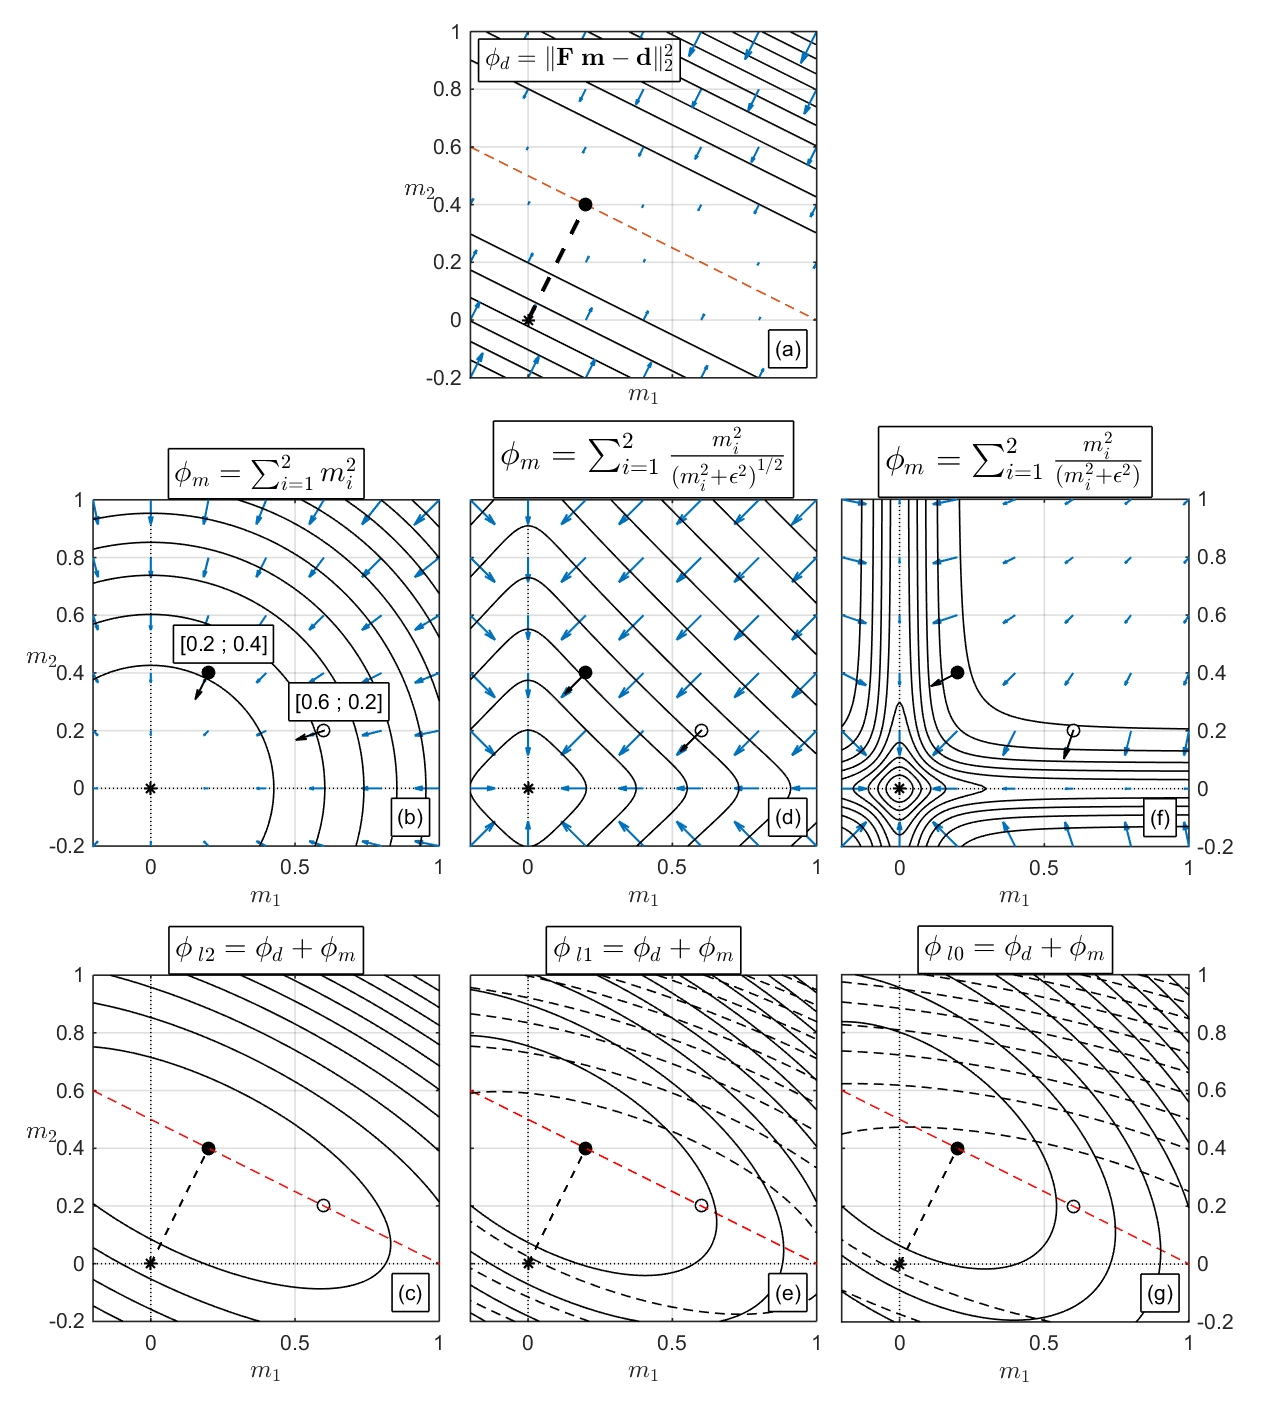
\includegraphics[scale=0.52]{IRLS_toy_l0l1l2}
\caption{Comparative contour maps for various objective functions over a range of model values $[ m_1 ;\;m_2 ]$. (a) The mininum of the misfit function $\phi_d$ forms a line spanned by $\mathcal{N} (\mathbf{F})$ (red dash). The $least-norm$ solution is marked as a solid dot. (Middle) Regularization functions and gradient directions (blue arrows) for approximated $l_p$-norm measures of the model for (b) $p=2$, (d) $p=1$ and (f) $p=0$.
The gradient directions are shown for two different starting models  (black arrows). 
(bottom) Contour maps of the initial objective functions $\phi(m) = \phi_d + \phi_m$ for the same two starting models: $\mathbf{m}^{(0)}_1$ (solid) and $\mathbf{m}^{(0)}_2$ (dash). (c) In the $l_2$-norm case , the function has a global minimum regardless of the starting model, while for non-linear functions for (e) $p=1$ and (g) $p=0$, the objective function changes with respect to the starting model.}
\label{fig:IRLS_toy}
\end{figure}

\begin{figure}[h!]
\centering
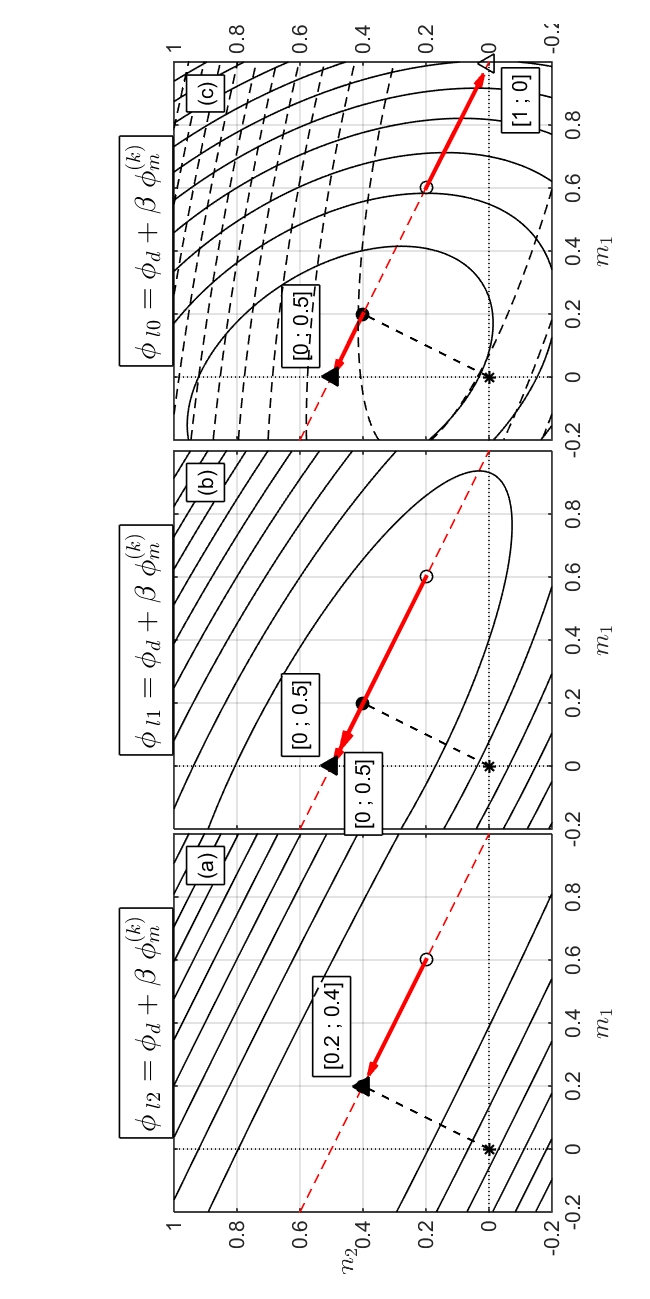
\includegraphics[scale=0.58,angle=270]{IRLS_toy_Result}
\caption{Contour maps for various objective functions after convergence of the IRLS algorithm. (a) Final model obtained with the $l_2$-norm penalty on the model for two starting models at $\mathbf{m}_1^{(0)}=[0.2;0.4]$ and $\mathbf{m}_2^{(0)}=[0.6;0.2]$ for a fixed trade-off parameter ($\beta = 1e-4$). In both cases, the solution converges to the global minimum, which is also the $least-norm$ solution at  $\mathbf{m_{ln}}=[0.2;0.4]$. 
(b) Solution with the $l_1$-norm penalty for the same starting models and trade-off parameter, converging to a global minimum at $\mathbf{m}^*=[0;0.5]$. This solution is sparse and can reproduce the data.
(c) The same experiment is repeated for the $l_0$-norm penalty, converging to two different solutions depending on the relative magnitude of the starting model parameters. Both solutions are sparse and honor the data. }
\label{fig:IRLS_toy_result}
\end{figure}

It is also important to note that the model norm regularization can be shifted away from the origin if we were to minimize:
\begin{equation}
\phi_m = \| \mathbf{m - m^{ref}} \|_2^2 \,.
\end{equation}
In this case, the minimum gradient of the objective function would occur at $\mathbf{m^{ref}}$. 
We would therefore look for a solution that both minimizes the data residual, while also approximating the expected model value. For simplicity, I consider the case where the reference model is at origin.

\section{$Lp$-norm and iterative re-weighted least squares} 
I have so far only considered the Euclidean norm of the model parameters,  penalizing the square of model values. 
Likewise, \cite{LiOldenburg1996} include an $l_2$-norm penalty on the model gradients, yielding smooth models.
In some cases, the solution may be expected to be sparse and blocky, either in terms of model parameters or spatial gradients. 
There have been several studies dedicated to the use of non-$l_2$ measures to recover models with sharp edges.
Most methods proposed in the literature made us of the globally convex $l_1$-norm, with proven convergence to a global minimizer \cite[]{FarquharsonOldenburg98, SunLi14, Daubechies10}.
Others have proposed approximations to the non-convex $l_0$-norm, methods such as the $compact$ regularization of \cite{ LastKubik83} and the $minimum\;support$ functional of \cite{Portniaguine1999}, to name a few.
My goal is to further generalize the proposed methods in order to explore a wide range of solutions for any combinations of $l_p$-norm penalty applied on the model and model gradients independently.

I begin with a generalized expression for the model objective function, such that \eqref{eq:obj_func} becomes:
\begin{equation} \label{eq:lpnorm}
\phi_m = \sum_{i=1}^{nc} \rho ( x_i ) \; ,
\end{equation}
where $\rho$ is some norm measure of a model function $\mathbf{x}(m)$ commonly chosen to be the model itself or some measure of spatial gradients. 
The general $l_p$-norm measure can be written as
\begin{equation} \label{eq:lpnorm}
\phi_m = \sum_{i=1}^{nc} {|x_i|}^p \;,
\end{equation}
where for $p=2$, I recover the standard regularized inversion presented in \eqref{eq:obj_func}.
Several approximations to the $l_p$-norm have been proposed, such as the Ekblom norm \cite[]{Ekblom73}: 
\begin{equation} \label{eq:Ekblom}
\phi_m =  \sum_{i=1}^{nc} {(x_i^2 + \epsilon^2)}^{p/2} \;,
\end{equation}
where a small number $\epsilon$ is added to guarantee that the function is continuous and differentiable as $\mathbf{x} \rightarrow 0$. 
Figure~\ref{fig:Lp_r_dphidm}(a) presents various norms for a fix threshold values ($\epsilon=1e-2$).
 The derivative of \eqref{eq:Ekblom} is given by:
\begin{equation} \label{eq:dphidm}
\begin{split}
\frac{\partial \phi_m}{\partial m} &= \sum_{i=1}^{nc} \rho'(x_i)  \frac{\partial x_i}{\partial m} \\
 &= p \;\frac{x_i}{{{(x_i}^{2} + \epsilon^2 )}^{1-p/2}}  \;  \frac{\partial x_i}{\partial m} \;.
\end{split}
\end{equation}
Expression \eqref{eq:dphidm} is clearly non-linear with respect to the model function $x_i$. 
As first introduced by \cite{Lawson61}, the norm can be linearized by the \emph{Iteratively Re-weighted Least-Squares} (IRLS) method such that:
 \begin{equation} \label{eq:IRLS_phi}
\phi_m^{(k)} =  \frac{1}{2}\sum_{i=1}^{nc} r_i \; x_i^2
\end{equation}
\begin{equation}\label{eq:IRLS_dphidm}
	\frac{\partial \phi_m^{(k)}}{\partial m}  =   r_i \; x_i \frac{\partial x_i}{\partial m} \;,
\end{equation}
where we added the superscript $\square^{(k)}$ to denote the IRLS iterations. The weights $r(x)$ are computed from model values obtained at a previous iteration such that:
\begin{equation}\label{eq:R_w}
	{r}_i  ={\Big( {({x_i}^{(k-1)})}^{2} + \epsilon^2 \Big)}^{p/2 - 1} \;,
\end{equation}
where ${r}(x) \in \mathbb{R}^{nc}$.

The goal of the IRLS method  is to approximate the $l_p$-norm by solving a series of locally convex least-squares problems.
The general objective function to be minimized takes the form:
\begin{equation}\label{eq:Lp_phi}
\begin{split}
\phi(m) &= \phi_d + \beta \phi_m^{(k)} \\
 &= \|\mathbf{ Fm - d }\|_2^{2} + \beta  \|\mathbf{ R\;x}(m) \|_2^{2} \;,
 \end{split}
\end{equation}
where the diagonal matrix $\mathbf{R} \in \mathbb{R}^{nc \times nc}$ holds the IRLS weights such that:
\begin{equation}
{R}_{ii} =  {{r}_i }^{1/2} \;.
\end{equation}
At each $k^{th}$ iteration, we seek a minimum along the gradient of the the objective function.
Replacing the regularization function from equation \ref{eq:dphi_dm} we get:
\begin{equation}\label{eq:dphi_dm_lp}
\begin{split}
 \mathbf{F^TF}\mathbf{m} + \beta\;\mathbf{g}(x) = \mathbf{F^T \; d} \\
\mathbf{g}(x) = \mathbf{R^TR\;x}(m) \frac{\partial \mathbf{x}(m)}{\partial m}\, ,
 \end{split}
\end{equation}
where I explicitly define the gradient of the approximated $l_p$-norm regularization function $\mathbf{g}(x)$.
I voluntarily neglect the constant of differentiation $p$ from equation \eqref{eq:IRLS_dphidm} for two reasons.
First, note that in the special case where $p=0$, the regularization function would vanish and reduce \ref{eq:dphi_dm_lp} to a simple least-squares problem.
Secondly, for any $p\ne0$, the constant would simply get absorbed by the trade-off parameter $\beta$.
Other parameters will be introduced in the following section to handle scaling issues arising from mixed-norm regularization functions.

Figure~\ref{fig:Lp_r_dphidm}(b) and (c) presents the IRLS weights $\mathbf{r}(x)$ and gradient functions $\mathbf{g}(x)$ for a range of $p$-value.
For $p=2$ and $\mathbf{x}(m) = \mathbf{m}$, we obtain the smooth regularization function presented in Figure~\ref{fig:IRLS_toy}(a).
It is important to note that for a small $l_p$-norm (i.e $p < 1$), the IRLS weights and gradients rapidly increase as $x_i \rightarrow \epsilon$.
The behavior of the regularization function around the threshold parameter $\epsilon$ is important for reasons that will be addressed in Section~\ref{eps_algo}.  

\begin{figure}[h!]
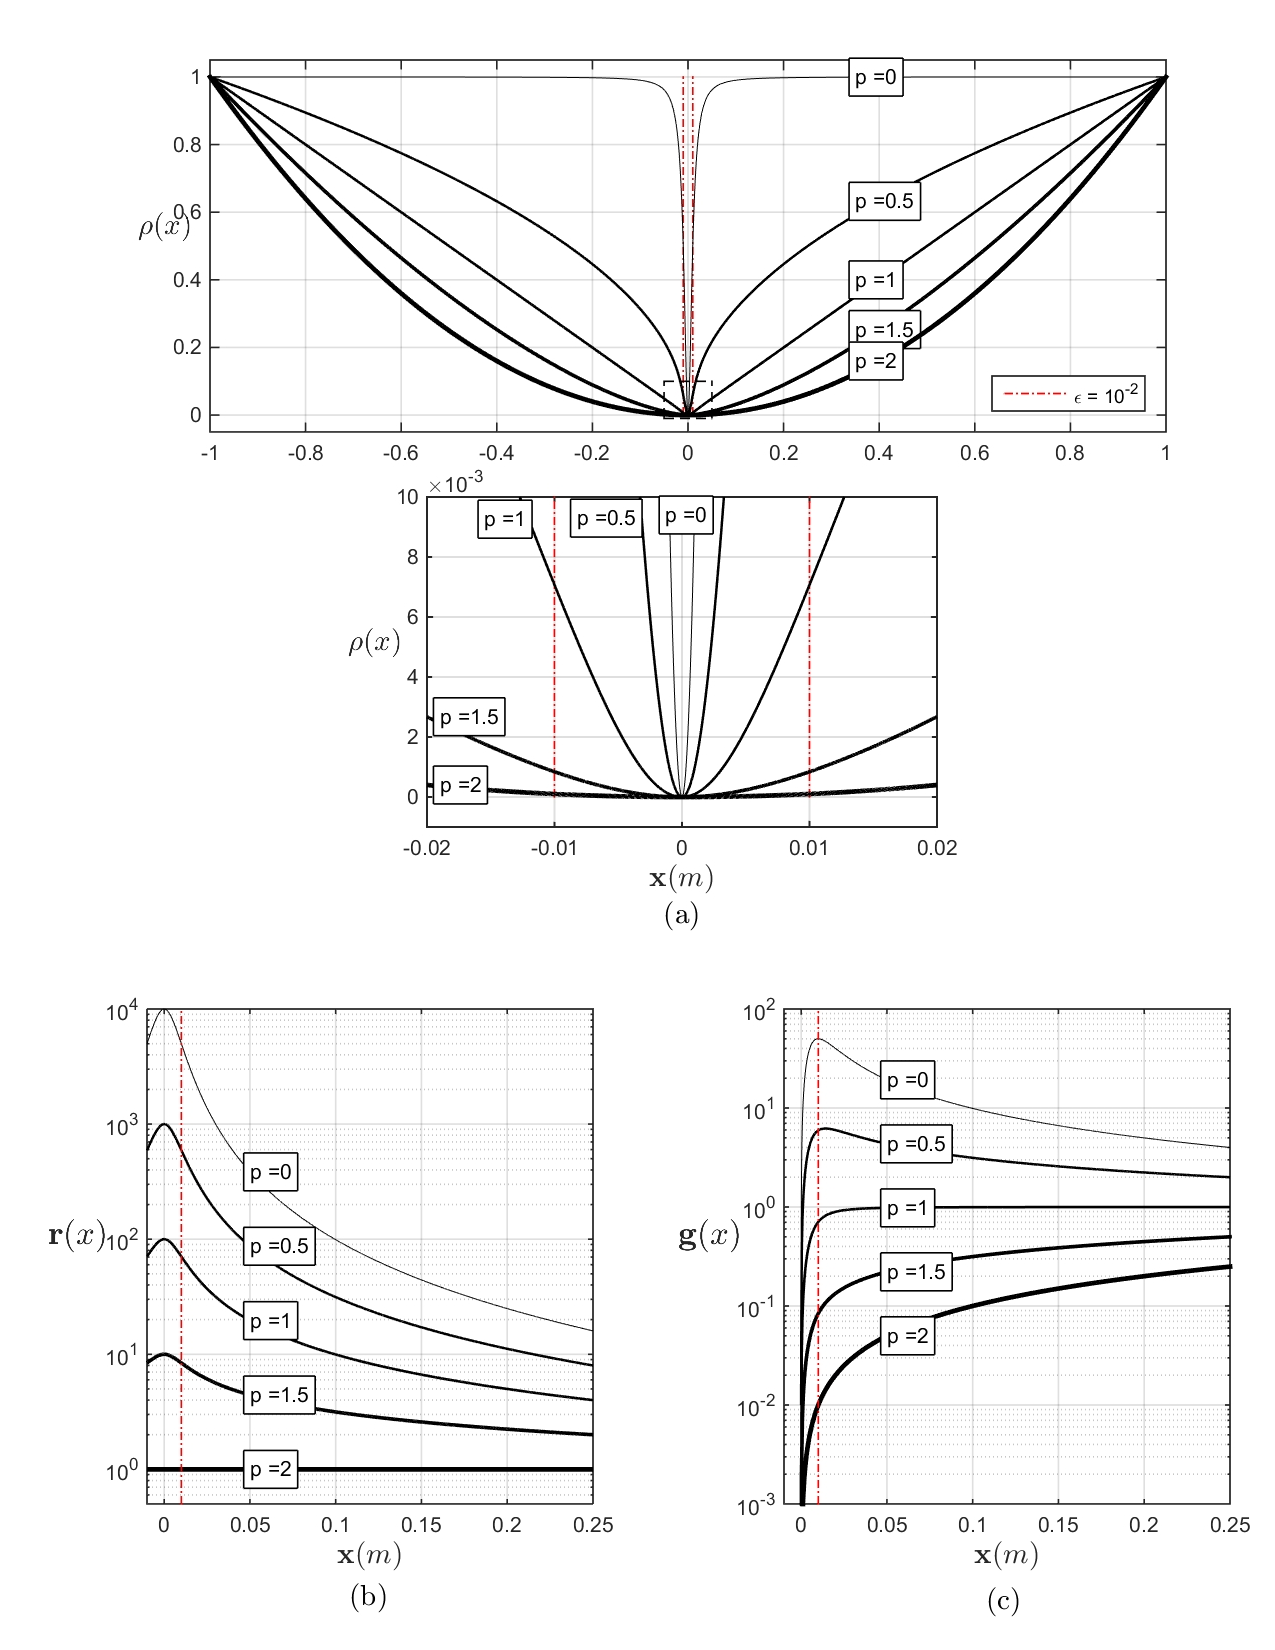
\includegraphics[scale=0.53]{Lp_r_dphidm}
\centering
\caption{(a) Penalty function $\rho(x)$ for different approximate $l_p$-norm measures, and enlarged view near the region of influence of $\epsilon$, making the $l_p$-norm continuous at the origin. (b) IRLS weights $\mathbf{r}(x)$ as a function of model function $\mathbf{x}(m)$ and $p$-values and for a fix threshold parameter ($\epsilon =1e-2$). (c)  Gradients $\mathbf{g}(x)$ of the model penalty function for various $p$-values. Note that the gradients are on a logarithmic scale due to the rapid increase as ${x}_i \rightarrow \epsilon$ for $p < 1$.}
\label{fig:Lp_r_dphidm}
\end{figure}

I illustrate the various $l_p$-norms on the same 2-variable inverse problem presented in Section~\ref{LN_and_RLS}.
Figure~\ref{fig:IRLS_toy}(d) and (e) show the regularization and the objective function for $p=1$, over a range of model parameters.
I point out that, compared to the globally convex $l_2$-norm, the shape of the objective function now depends on the starting model $\mathbf{m_1}^{(0)}$ and $\mathbf{m_2}^{(0)}$.

For $p = 0$, I recover the \textit{compact} regularization function put forward by \cite{ LastKubik83}, which has been borrowed by many researchers in geophysics \cite{BarbosaSilva94, Ajo-Franklin07, Stocco09}.
Figure~\ref{fig:IRLS_toy}(f) and (g) presents the approximated $l_0$-norm and corresponding objective function over the same range of model parameters. 
Similarly, the minimum of the objective function depends on the initial model $\mathbf{m}^{(0)}$ used to construct the regularization.

Although difficult to prove analytically, experiments have shown that the $l_0$-norm can yield a sparser solution than the convex $l_1$-norm \cite[]{Chartrand07}. 
I use the same 2-variable example to illustrate this idea.
For simplicity, I impose a fix threshold parameter ($\epsilon = 1e-8$) and a fix trade-off parameter ($\beta=1e-4$).
%\textemdash two small values found empirically to approximate the norm well while minimizing the data misfit. 
Here, I am only interested in the final solution depending on the choice of $l_p$-norm, and as a function of starting model $\mathbf{m}^{(0)}$. 
In the next section, I will provide strategies to efficiently determine those parameters.

In the first experiment, I choose the starting model $\mathbf{m_1}^{(0)}$ to be the least-norm solution at $\mathbf{m_{ln}}$= [0.2;0.4], marked as a solid dot (Fig.~\ref{fig:IRLS_toy_result}). 
In both cases the $l_1$-norm and $l_0$-norm converge to the same optimal solution at $\mathbf{m^{*}}$= [0.0;0.5].
The model $\mathbf{m^{*}}$ is interesting as it is sparse with a single non-zero parameter, while also having the smallest norm possible.

In the second experiment, the initial model is also chosen to satisfy the target data misfit, but this time with a relatively smaller value on the second variable such that $\mathbf{m_2}^{(0)}$= [0.6;0.2], marked as a white dot. 
Because both the $l_1$-norm and $l_0$-norm penalize small model parameters, the regularization forces the solution to be sparse along $\mathcal{N} (\mathbf{F})$. 
Note the clear difference between the globally convex $l_1$-norm, converging back to $\mathbf{m^{*}}$, compared to the non-convex $l_0$-norm, reaching the $m_1$-axis at $\mathbf{m}^{(k)}$= [1;0]. 
The $l_0$-norm has therefore two possible solutions that do not depend on the overall magnitude of $\mathbf{m}^{(0)}$, but rather on the \emph{relative} magnitude of its components $[m_1\;;\;m_2]$. 
The $l_0$-norm acts as a binary selector, influenced by the largest elements of a starting model.

The choice of specific norm should therefore reflect the expected character of the solution, and the chosen algorithm should allow access to the full range of norms for $0\leq p \leq 2$.
While it is simple to solve \eqref{eq:Lp_phi} for a 2-variable problem, finding a solution to large systems for non-convex norms ($p < 1$) has proven to be difficult and remains a field of active research. 
%\cite[]{ PortniaguineZhdanov02, Ajo-Franklin07, SunLi14, Stocco09, BarbosaSilva94}. 
The following sections review potential complications for the non-convex cases, and review strategies to efficiently solve the IRLS method.

%%%%%%%%%%%%%%%%%%%%%%%%%%%%%%%
\section{IRLS solver}\label{Solve_IRLS}
The IRLS method presented in \ref{eq:Lp_phi} is an iterative process, which depends on two key parameters: the trade-off parameter $\beta$ and the threshold parameter $\epsilon$.
In this section, I explore four strategies for the implementation of the IRLS.

\subsection{Basic IRLS algorithm}
As illustrated with the previous 2-variable problem, the choice of a starting model $\mathbf{m}^{(0)}$ is especially important for non-convex norms $p < 1$.
According to \cite{Chartrand07}, it may be possible to compute a global minimizer from non-convex functions, as long as the initial model is close enough to the global optimum.
Most methods proposed in the literature seem to agree on the $l_2$-norm solution as a valid candidate \cite[]{ PortniaguineZhdanov02, Ajo-Franklin07, SunLi14}.
Current inversion strategies already rely on the assumption that a smooth model is a good approximation of the true solution.
Applying a sparse $l_p$-norm can then segregate the most important model parameters, which in turn can reduce the complexity of the solution. 
This is mostly interesting if the true solution is known to behave like a delta function. 

The basic IRLS algorithm becomes a two step process, as summarized in Table~\ref{tbl:IRLS_v1}.
During Phase-I, the algorithm finds a smooth solution with the $l_2$-norm regularization.
The trade-off parameter $\beta$ is monotonically reduced until the model can predict the data near the target misfit $\phi_d^*$.
The final $l_2$-norm solution provides a starting model $\mathbf{m}^{(0)}$ for the calculation of a weighting matrix $\mathbf{R}$.

In Phase-II of the IRLS method, model updates are computed iteratively by minimizing \ref{eq:Lp_phi}.
This process is repeated until the algorithm converges to a stable solution.
I define a $convergence$ criteria as:
\begin{equation}\label{Convergence}
\begin{split}
\delta \phi_m^{(k)} & = \frac{|\phi_m^{(k)} - \phi_m^{(k-1)}|}{\phi_m^{(k)}} \times 100\% \;,
\end{split} 
\end{equation} 
where the change in model norm falls below some pre-defined threshold, chosen to be 2\% in all my experiments.
In the simplest form of the algorithm, the threshold $\epsilon$ and trade-off parameter $\beta$ remain constant throughout Phase-II.
For now, I will follow the general consensus that $\epsilon$ has to be small, or near machine error ($\epsilon_p = \epsilon_q = 1e-8$) \cite[]{LastKubik83,Ajo-Franklin07, Stocco09}.
I will revisit this number in Section~\ref{eps_algo}.
In the method proposed by \cite[]{Ajo-Franklin07}, a trade-off parameter $\beta^*$ is chosen so that the initial IRLS solution predicts the data near the target misfit $\phi_d^*$. 
This $\beta^*$ then remains constant throughout the iterative process.

\begin{table}[h!]
\centering
\caption{IRLS Solver 1: Fix parameters}
\label{tbl:IRLS_v1}
\renewcommand{\arraystretch}{1.5}
\begin{tabular}{|c|}\hline
\textbf{Phase I - $L_2$-norm iterations:  $\left\{ \mathbf{m}^{(0)} \mid \phi_d \simeq \phi_d^* \right \}$}\\
Adjust $\beta$ \\
$min\; \phi(m)  \rightarrow \mathbf{m}^{(0)}$ \\ \hline
Search:   $\left\{  \beta^* \mid \phi_d^{(k)} \simeq \phi_d^* \right \}$\\ \hline
\textbf{Phase II - $L_p$-norm iterations: $\left\{  \mathbf{m}^{(k)} \mid \delta \phi_m^{(k)} < 1\%  \right \}$ }\\
Fix \{$\beta^*, \epsilon_p,\epsilon_q$\}\\
Update $r_i^{(k)}$\\
$min\; \phi^{(k)}  \rightarrow \mathbf{m}^{(k)}$\\ \hline
\end{tabular}
\end{table}

\subsection{1-D synthetic example}
I demonstrate this simple IRLS implementation on a synthetic 1D problem similar to the problem used by \cite{LiOldenburg1996}.
The model consists of a rectangular pulse and a Gaussian function on the interval [0 1] and discretized with 200 uniform intervals. Data are generated from the equation:
\begin{equation} \label{eq:9}
  d_j = \int_0^1 f_j(x) m(x) \; dx, \:\: j = 0, ..., N\;,
\end{equation}
where the kernel functions relating the model and the data are defined as:
\begin{equation} \label{eq:kernel_1D}
  f_j(z) = e^{-j\:x }\cdot cos(2 \pi j x) \;,
\end{equation}
where $x$ defines the distance along the $x$-axis. 

The model and kernel functions for $j \in [1 , 30]$ are shown in Figure \ref{fig:1D_model}. 
Two percent random noise is added to the data in order to simulate a true geophysical experiment. 
The data are weighted accordingly such that:
\begin{equation} \label{eq:Weighted_misifit}
	\phi_d = \|\mathbf{W_d \;( F\;m - d)}\|_2^{2}\;,
\end{equation}
where the diagonal matrix $\mathbf{W_d}$ holds the estimated uncertainties associated with each datum. 
Since the noise is assumed to be Gaussian and uncorrelated, the misfit function follows a chi-squared distribution with expected value of $N$, hence the target misfit.

\begin{figure}[h!]
\centering
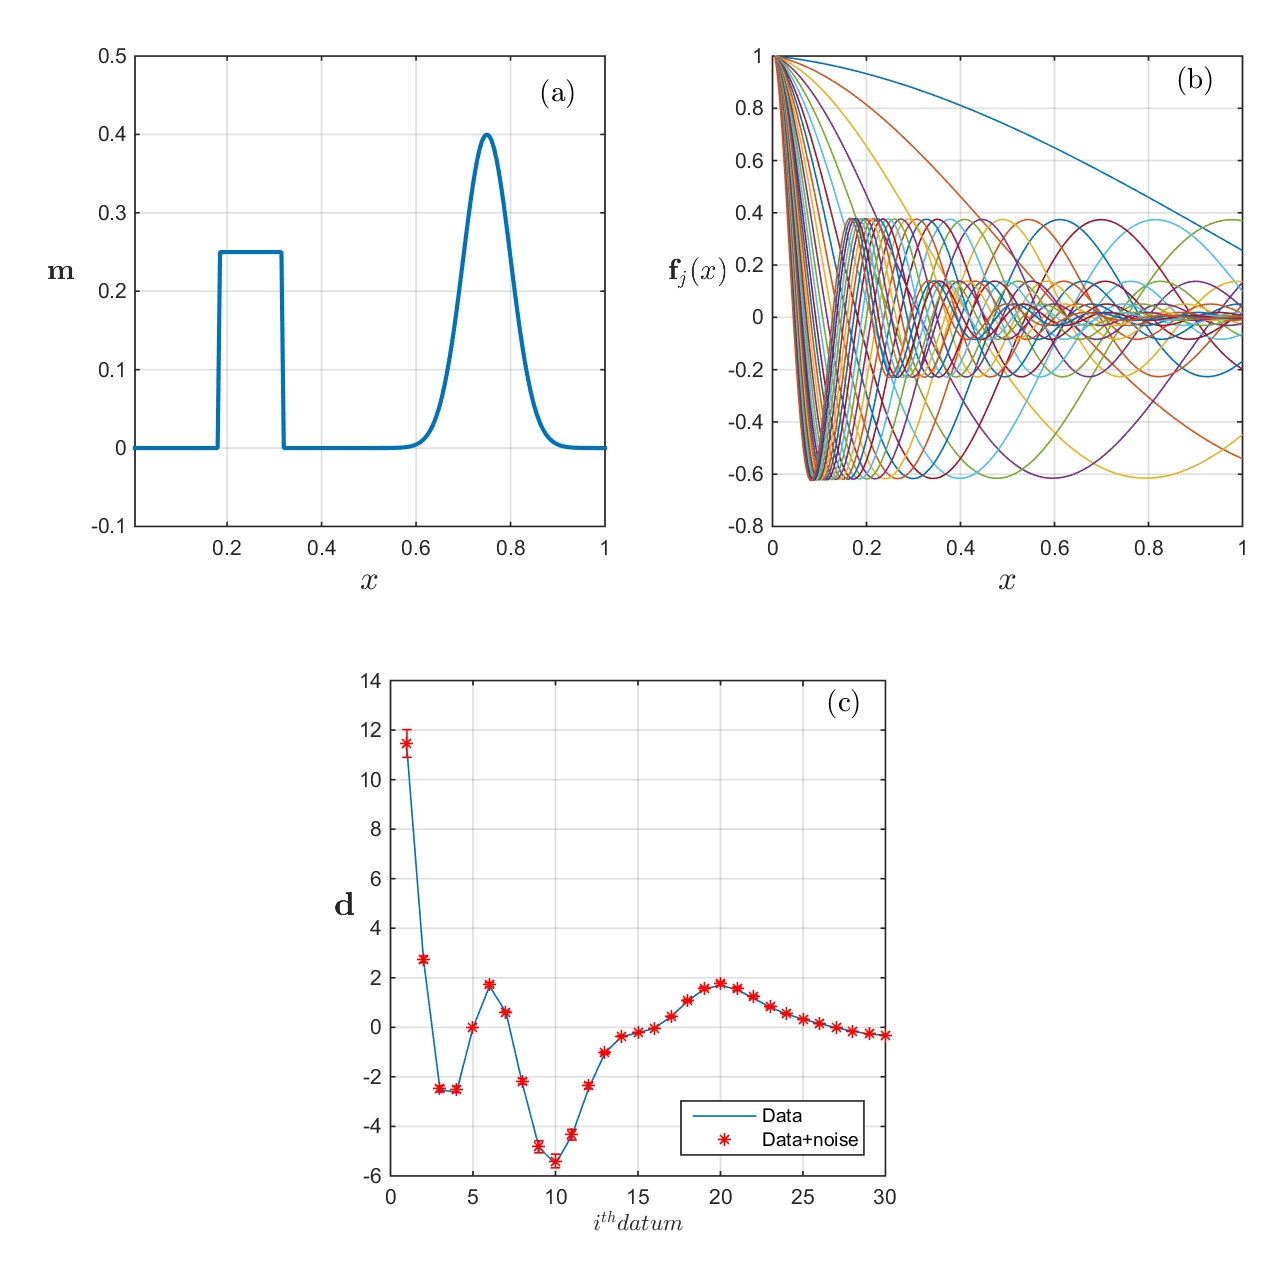
\includegraphics[scale=0.55]{1D_Kernel_data}
\caption{(a) Synthetic 1D model made up of a rectangular pulse and a Gaussian function. (b) Kernel functions consisting of exponentially decaying cosin functions of the form $ f_j(x) = e^{-j\:x }\cdot cos(2 \pi j x)$. (c) Data generated from $\mathbf{d =F \; m}$ , with $5\%$ random  Gaussian noise added. }
\label{fig:1D_model}
\end{figure}

I here generalize the objective function presented in Chapter~\ref{ch:Chap3_Inverse} to allow for multiple $l_p$-norm regularization functions such that:
\begin{equation} \label{eq:Lp_phi_int}
\phi(m) =  \phi_d + \beta \Big [ \int_0^1 w_s \; {\left|m - m^{ref}\right|^p} \; dl + \int_0^1 w_x\; {\left|\frac{\partial m}{\partial x}\right|^{q}} \;dl \Big ]\;.
\end{equation}
The only difference with the regularization function used in \ref{eq:Phi_int} is in the norms applied on the model and model gradients ${|\cdot|}^p$ and ${|\cdot|}^q$, where $p$ and $q$ can take any value on the interval $[0, 2]$.
Since we are dealing with a 1-D problem, model gradients are only computed along the $x$-axis.
I also apply a depth weighting function to counter the decay of the kernel functions such that:
\begin{equation}\label{DepthWeight}
\begin{split}
w_s = \alpha_s\; e^{jx}\\
w_x = \alpha_x\; e^{jx}\;.
\end{split}
\end{equation}
Combining the IRLS approximation in \eqref{eq:Lp_phi} and the discrete objective function presented in \ref{eq:Phi_disc}, the linear 1-D equation \ref{eq:Lp_phi_int} becomes:
 \begin{equation} \label{eq:Lp_phi_1D}
\phi(m) =  \|\mathbf{W_\text{d} \;( F\;m - d)}\|_2^{2} + \beta \Big [ {\| \mathbf{W}_s \; \mathbf{R}_s\; ( \mathbf{m - m^{ref}})\|}^2_2  + {\|   \mathbf{W}_x  \; \mathbf{R}_x\; \mathbf{G}_x \; \mathbf{m}\|}^2_2  \Big ]\;,
\end{equation}
where the diagonal matrices $\mathbf{W}_s,\mathbf{W}_x$ are the cell weights, and $\mathbf{G}_x$ is the spatial gradient operator presented in Chapter~\ref{ch:Chap3_Inverse}.
The IRLS weights $\mathbf{R}_s$ and $\mathbf{R}_x$ are defined as:
\begin{equation}\label{eq:Rs_Rx}
\begin{split}
	{R}_{s_{ii}}  &= {\Big[ {({m_i}^{(k-1)})}^{2} + \epsilon_p^2 \Big]}^{(p/2 - 1)/2} \\
	{R}_{x_{ii}}  &= {\Big[ {\left ({\frac{\partial m_i^{(k-1)} }{\partial x}}\right)}^{2} + \epsilon_q^2 \Big]}^{(q/2 - 1)/2}  \;,
\end{split}
\end{equation}
where $\epsilon_p, \epsilon_q$ are the stabilizing parameters for the sparsity constraint applied on the model and model gradient respectively.

As explained in Section \ref{Iterative solver}, the minimum norm solution is found where $\frac{\partial \phi(m)}{\partial m} = 0$.
Taking the partial derivatives of \ref{eq:Lp_phi_1D} with respect to the model parameters and setting the reference model to zero yields:
\begin{equation}\label{eq:dphi_dm_inv}
\Big ( \mathbf{F^TW_\text{d}^TW_\text{d}F} + \beta \big [ \mathbf{R}_s^{\mathbf{T}}\; \mathbf{W}_s^{\mathbf{T}} \mathbf{ W}_s \;\mathbf{ R}_s + \mathbf{G}_x^{\mathbf{T}} \;\mathbf{R}_x^{\mathbf{T}}\; \mathbf{W}_x^{\mathbf{T}}\mathbf{ W}_x \;\mathbf{R}_x \; \mathbf{G}_x \; \big]\Big ) 
\mathbf{m = F^TW_\text{d}^TW_\text{d}d} \;.
\end{equation}
This linear system can be expressed as an overdetermined problem of the form:
\begin{equation}\label{eq:lsqr_IRLS_dphi_dm}
 \begin{bmatrix}
\mathbf{W_\text{d}} \;\mathbf{F} \\
\sqrt{\beta} \mathbf{W}_s \;\mathbf{R}_s\\
\sqrt{\beta} \mathbf{W}_x \;\mathbf{R}_x \;\mathbf{G}_x \\
 \end{bmatrix} \mathbf{m} =
   \begin{bmatrix}
\mathbf{W_\text{d}} \; \mathbf{d}\\
0 \\
0
 \end{bmatrix} \;.
 \end{equation}
Solving the least-squares problem \ref{eq:lsqr_IRLS_dphi_dm} yields a model update at the $k^{th}$ iteration of the IRLS method.
In this case, the left-hand side of \ref{eq:dphi_dm_inv} is linear with respect to $\mathbf{m}^{(k)}$ and it forms a symmetric positive definite matrix, which can be solved efficiently by the Conjugate Gradient descent method.

For the initial phase of the IRLS method, a solution is found with the globally convex $l_2$-norm regularization, in which case $\mathbf{R}_s$ and $\mathbf{R}_x$ reduce to the identity matrix.
Figure \ref{fig:1D_IRLS_algo1}(a) presents the inverted result obtained with the $l_2$-norm, as well as the convergence curve after achieving the target data misfit $\phi_d^*$. 
As expected from an $l_2$-norm regularization, the solution is smooth and dispersed over the entire model domain.

\begin{figure}[p]
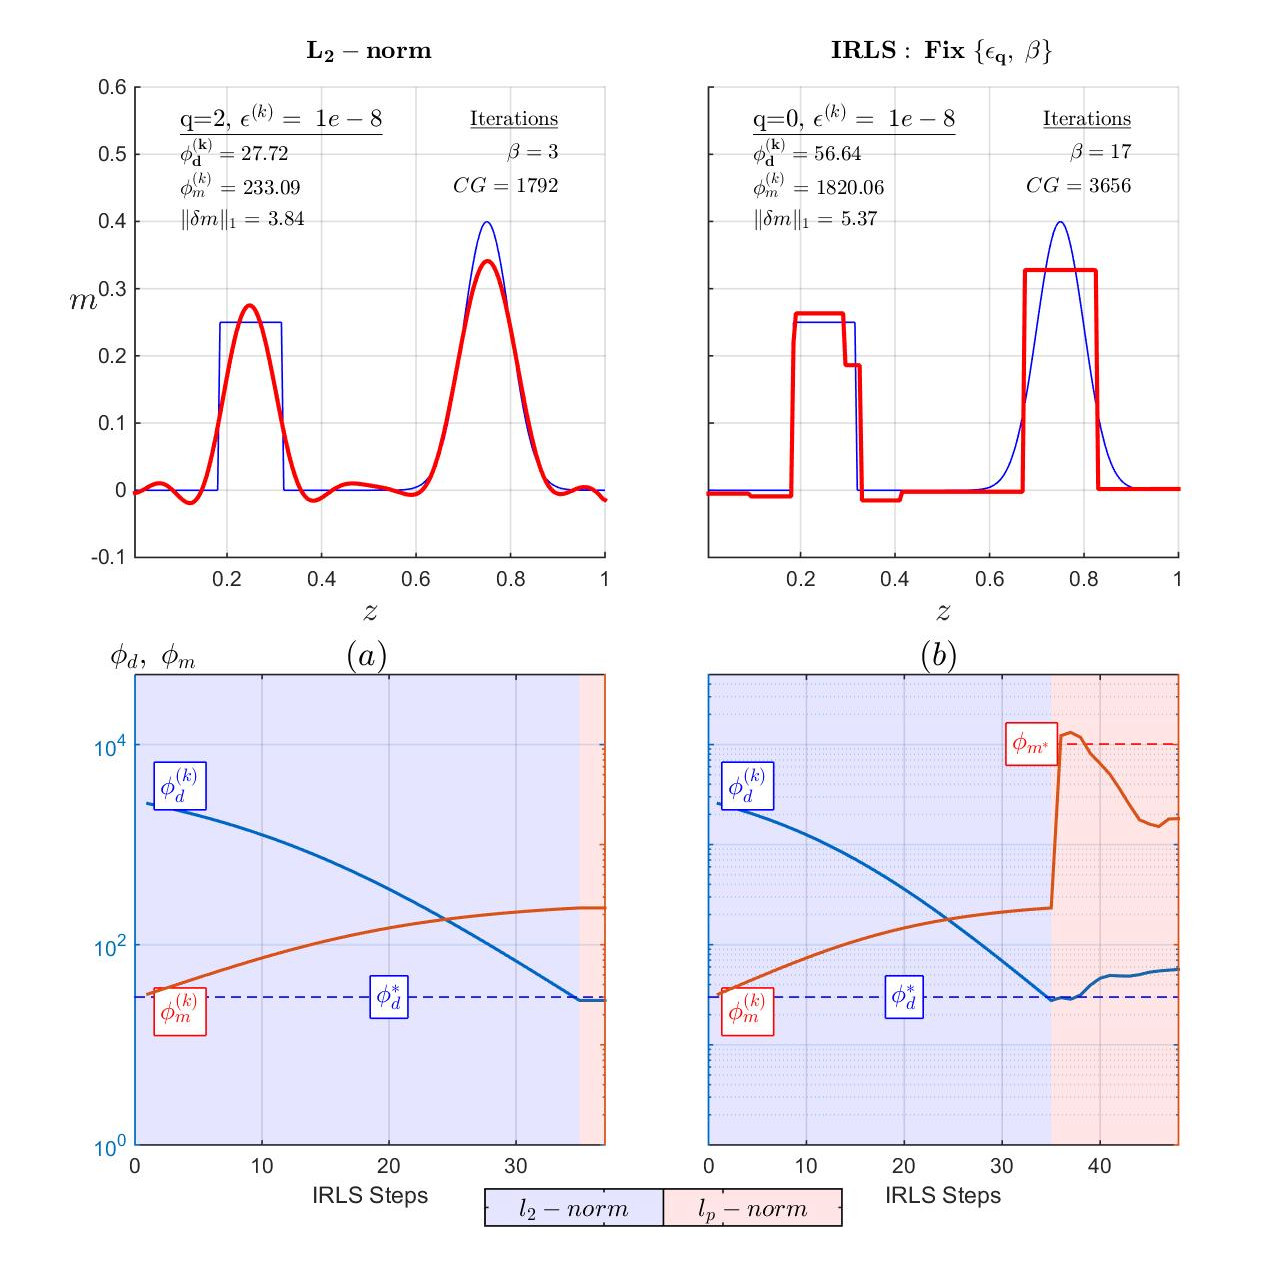
\includegraphics[scale=0.6]{1D_IRLS_algo1}
\caption{(a) Recovered models from the smooth $l_2$-norm regularization, and (bottom) measure of model misfit and model norm as a function of iterations. Both the rectangular pulse and Gaussian function are recovered at the right location along the $x$-axis, but the solution is smooth and dispersed over the entire model domain. (b) Solution obtained from the IRLS with spasity constraints on the model gradients ({q=0}), using the $l_2$-norm model (a) to initiate the IRLS steps. The algorithm uses a fixed threshold parameter ($\epsilon=1e-8$) and fixed trade-off parameter $\beta$. The final solution is blocky, as expected from the norm chosen, but fails to achieve the target data misfit. Clearly the influence of the regularization function has overtaken the minimization process.}
\label{fig:1D_IRLS_algo1}
\end{figure}

From there, the algorithm proceeds with a sequence of IRLS iterations with $l_0$-norm penalty on the model gradient ($\alpha_s=0, q =0$).
The goal is to use the regularization to enforce a solution with sharp gradients and hopefully recover the rectangular pulse.
The IRLS weights are initiated with the smooth $l_2$-norm solution.
The initial $\beta^*$ is found by a search method where a solution to equation~\ref{eq:lsqr_IRLS_dphi_dm} is computed for multiple trials.
The iterative process is repeated until the inversion reaches the convergence criteria specified by equation~\ref{Convergence}, while keeping the trade-off parameter $\beta^*$ constant.

As shown in Figure~\ref{fig:1D_IRLS_algo1}(b), the updated solution with the $l_0$-norm penalty recovers a blocky model with sharp edges. 
It is important to note that the final data residual $\phi_d^{(k)}$ is much larger than the target misfit ($\phi_d^*=30$).
Clearly the influence of the regularization has overtaken the inversion process.
The algorithm likely converged to some local minimum, far from the global optimizer previously found with the smooth $l_2$-norm.
Since I know the true solution, I can measure the accuracy of the solution, or model error as:
\begin{equation}
\| \delta m \|_1 = \sum_{i = 1}^{nc} |m_i^{(k)} - m_i^*| \;,
\end{equation}
where $\mathbf{m}^{(k)}$ is the solution found at the $k^{th}$ iteration.
The final model error is larger than the one found with the smooth $l_2$-norm regularization, hence it is a poor estimate of the true solution.

This example clearly illustrates some of the challenges related to non-convex objective functions.
We have so far only formulated the basic algorithm behind the IRLS method, which has been used by many researchers in the past.
Important details regarding the stability and predictability of the algorithm will now be addressed.

\subsection{Regularization scaling}
Following Tikhonov's approach, a solution to the inverse problem is found by progressively reducing the influence of the regularization until reaching the target data misfit $\phi_d^*$. 
For strictly convex regularization functions, such as the $l_2$-norm, the influence of the regularization functions is scaled linearly by the trade-off  parameter $\beta$. 
For non-convex functions, in our case for $q = 0$, the iteration process involves non-linear transformations of the objective function, driven by the IRLS weights computed in \eqref{eq:R_w}. 
Those weights can change rapidly as $\epsilon \rightarrow 0$, which directly impacts the influence of the model norm in a non-linear fashion. 
As demonstrated in Figure~\ref{fig:1D_IRLS_algo1}(b), special care must be taken in order to obtain a solution that satisfies the data while also being sparse.

As a second strategy, I experiment with a brute-force approach where the optimal trade-off parameter $\beta$ is determined before each IRLS steps (Table~\ref{tbl:IRLS_v2}).
A solution to \ref{eq:dphi_dm_lp} is computed several times for a range of $\beta$-values until a suitable trade-off parameter is found.
Figure~\ref{fig:1D_IRLS_algo2}(a) presents the model and convergence curve following this strategy.
The solution is blocky, as expected from the $l_0$-norm on model gradients, while also honoring the data within $1\%$ of the target misfit.
This iterative process is very expensive however, as it requires multiple $\beta$ solves per IRLS iteration.
For large non-linear problems, this type of approach would be computationally prohibitive.

\begin{table}[h!]
\centering
\caption{IRLS Solver 2: $\beta$-search}
\label{tbl:IRLS_v2}
\renewcommand{\arraystretch}{1.5}
\begin{tabular}{|c|}\hline
\textbf{Phase I - $L_2$-norm iterations:  $\left\{ \mathbf{m}^{(0)}, \beta^{(0)} \mid \phi_d \simeq \phi_d^* \right \}$}\\
Adjust $\beta$ \\
$min\; \phi(m)  \rightarrow \mathbf{m}^{(0)}$ \\ \hline
\textbf{Phase II - $L_p$-norm iterations: $\left\{  \mathbf{m}^{(k)} \mid \delta \phi_m^{(k)} < 1\% \right \}$ }\\
Fix \{$\epsilon_p,\epsilon_q$\}\\
Update $r_i^{(k)}$\\
Search:   $\left\{  \beta^{(k)} \mid \phi_d^{(k)} \simeq \phi_d^* \right \}$\\
$min\; \phi^{(k)}  \rightarrow \mathbf{m}^{(k)}$\\ \hline
\end{tabular}
\end{table}

\begin{figure}[p]
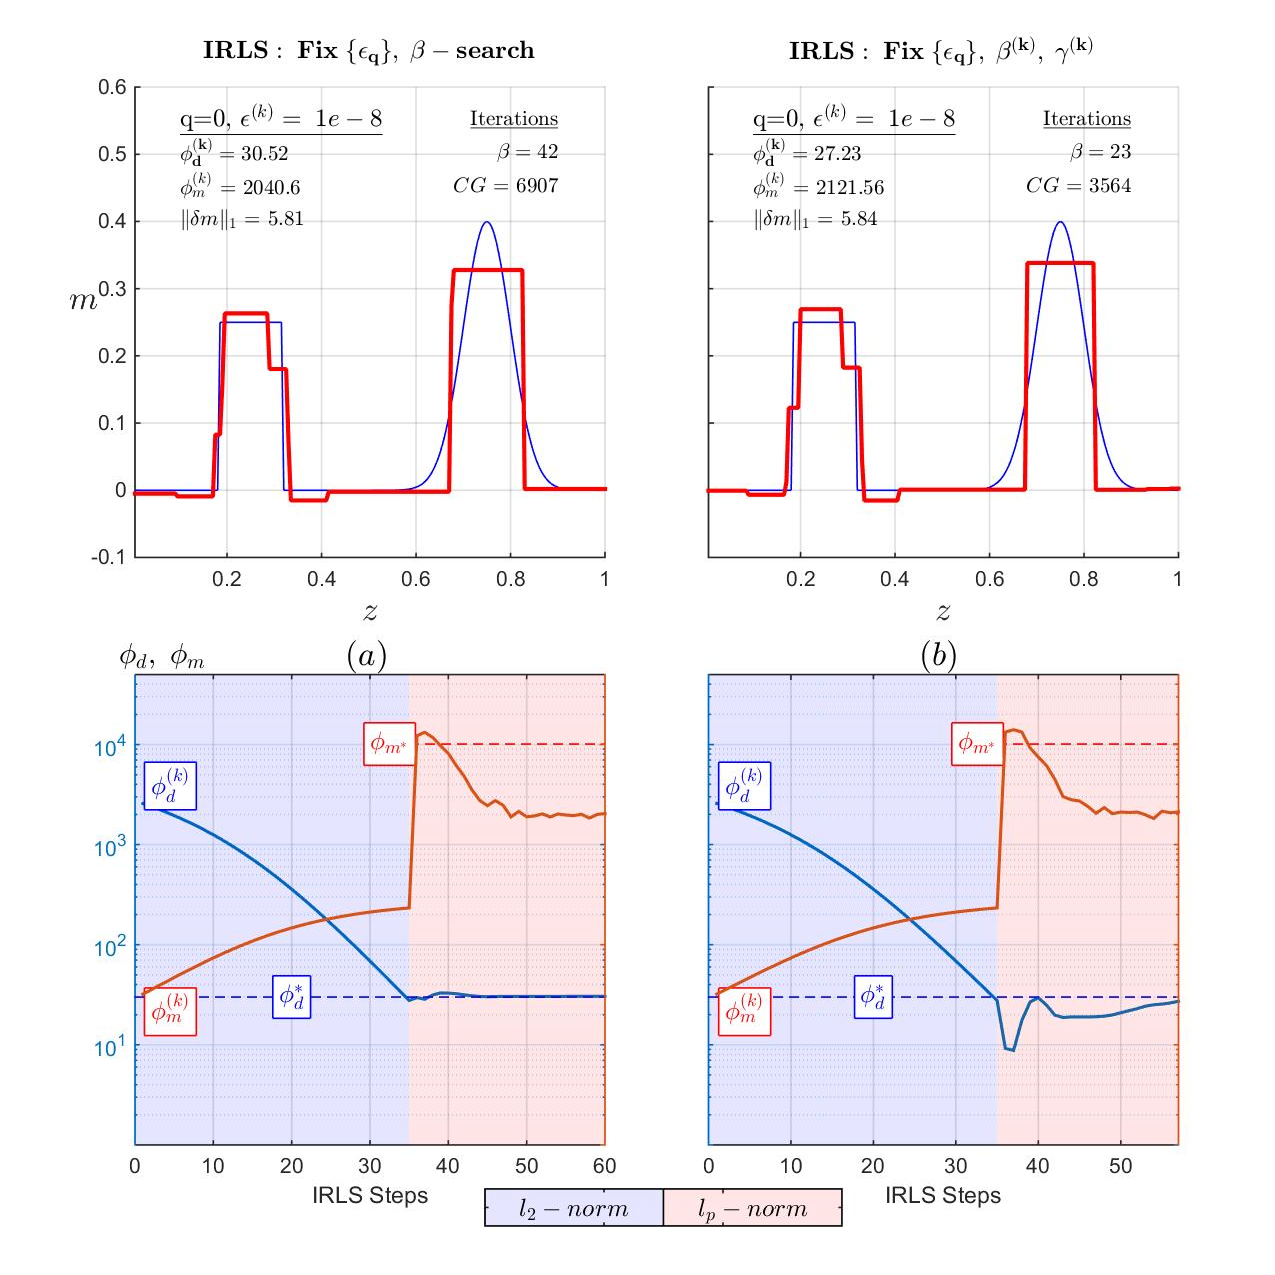
\includegraphics[scale=0.6]{1D_IRLS_algo2}
\caption{(Top) Recovered models from two different algorithms used to implement the IRLS method for $q=0$ and a fix threshold parameter ($\epsilon=1e-8$). (Bottom) Measure of model misfit and model norm as a function of iterations. (a) The first algorithm searches for an optimal trade-off parameter $\beta^{(k)}$ between each IRLS step, requiring a solution to multiple sub-inversions. (b) The second algorithm only adjusts $\beta^{(k)}$ once after each IRLS step. A new scaling parameter $\gamma^{(k)}$ is added to smooth the transition between the IRLS updates. The algorithm recovers a similar blocky model but is computationally cheaper, as indicated by the total number of beta iterations and CG solves.}
\label{fig:1D_IRLS_algo2}
\end{figure}

As a third strategy, I relax the requirement for the model to predict the data $exactly$ between each IRLS steps. 
The trade-off parameter is adjusted once after each IRLS step such that:
\begin{equation}
\beta^{(k+1)} = \beta^{(k)} * \frac{\phi_d^*}{\phi_d^{(k)}} \;.
\end{equation}
I have found experimentally however that this type of posterior update is not sufficient to guarantee a smooth convergence. 
The initial IRLS update can change the model substantially, moving away from the global $l_2$-norm solution. 
In order to preserve the relative importance between misfit and regularization functions while reducing the computational cost, I propose an iterative re-scaling of the model objective function such that:
\begin{equation}\label{eq:scaled_Lp_phi}
\begin{split}
\hat \phi_m^{(k)} = \gamma^{(k)} & \Big ( {\| \mathbf{W_\text{s} \; R_\text{s} \; m}\|}^2_2 +  {\|  \mathbf{ W_\text{x}\; R_\text{x} \; G_\text{x} \; m}\|}^2_2  \Big ) \\
 \gamma^{(k)}  &= \frac{\hat \phi_m^{(k-1)}}{  {\| \mathbf{W_\text{s} \; R_\text{s} \; m}^{(k-1)}\|}^2_2 + {\|  \mathbf{W_\text{x}\; R_\text{x} \; G_\text{x} \; m}^{(k-1)}\|}^2_2 }\;,
 \end{split}
\end{equation}
where $\phi_m^{(k)}$ is the scaled model objective function at some $k^{th}$ iteration, and $\gamma^{(k)}$ is a scalar computed at the beginning of each IRLS iterations. 
Effectively we are searching  for model parameters that are close to the present solution.
Since we are changing the $rule$ by which the size of the model is measured, we attempt to account for it. 
I point out that for constant $l_p$-norm regularizations, the scaling parameter $\gamma^{(k)}$ is equal to one.
Table~\ref{tbl:IRLS_v3} summarizes the proposed method.

\begin{table}[h!]
\centering
\caption{IRLS Solver 3: Scaled regularization}
\label{tbl:IRLS_v3}
\renewcommand{\arraystretch}{1.5}
\begin{tabular}{|c|}\hline
\textbf{Phase I: $L_2$-norm iterations  $\left\{ \mathbf{m}^{(0)}, \beta^{(0)} \mid \phi_d \simeq \phi_d^* \right \}$}\\
Adjust $\beta$ \\
$min\; \phi(m)  \rightarrow \mathbf{m}^{(0)}$ \\ \hline
\textbf{Phase II: $L_p$-norm iterations $\left\{  \mathbf{m}^{(k)} \mid \delta \phi_m^{(k)} < 1\%,\; \phi_d \simeq \phi_d^* \right \}$ }\\
Fix \{$\epsilon_p,\epsilon_q$\}\\
Update $r_i^{(k)}$\\
Scale $\hat \phi_m^{(k)}$ \\
$min\; \phi^{(k)}  \rightarrow \mathbf{m}^{(k)}$\\ 
$\beta^{(k+1)}=\beta^{(k)} *\frac{\phi_d^*}{\phi_d^{(k)}} $\\ \hline
\end{tabular}
\end{table}
As shown in Figure \ref{fig:1D_IRLS_algo2}(b), the re-scaling procedure greatly reduces the total number of CG solves. 
Even though nothing guarantees that non-convex norms will converge to a $global$ minimum, the re-scaling scheme proposed here forces local minima to be in the proximity of the $l_2$-norm solution.
In other words, the scaling parameter $\gamma^{(k)}$ helps preserve the character of all previous iterations, slowly converging to a new minimum, hopefully in the vicinity of the global $l_2$-norm solution.

\subsection{Threshold parameter $\epsilon$}\label{eps_algo}
I have so far delayed providing details regarding the choice of threshold parameter $\epsilon$, which has been the subject of disagreement among researchers \cite[]{LastKubik83, BarbosaSilva94, Ajo-Franklin07, Stocco09, SunLi14}.  
Little has been said in the literature on how to determine a specific value of $\epsilon$.

In the classic work of \cite{LastKubik83}, and many other research papers after, it has been suggested that the stabilizing parameter should be small ($\epsilon < 10^{-8}$), or near machine error in order to approximate the $l_p$-norm well. 
Other researchers, such as in \cite{Ajo-Franklin07} have observed severe instabilities with such a small value, and found experimentally that $\epsilon$ should be between $10^{-4}$ and $10^{-7}$.
This may be due to the large spread in weights along the diagonal of \textbf{R} impacting the conditioning of the linear system described in equation \eqref{eq:dphi_dm}. A large condition number can adversely affect the convergence rate of gradient descent solvers.

As an alternative to the regularization function used by \cite{ LastKubik83}, \cite{Gorodnitsky97} apply the IRLS weights directly to the sensitivity matrix . The general objective function to be minimized takes the form:
\begin{equation}\label{eq:Lp_Jweighted}
 \phi = \|\mathbf{ \hat F \hat m - d }\|_2^{2} + \beta \|\mathbf{ \hat x}(m) \|_2^{2} \;,
\end{equation}
where the weighted forward model operator is written as:
\begin{equation}\label{eq:m_weighted}
 \mathbf{ \hat F = F}\;diag[\mathbf{m}^{(k-1)}]\;.
\end{equation}
The same technique was later revised by \cite{Portniaguine1999, PortniaguineZhdanov02} and coined Minimum Support (MS) functional.
The method was extended to penalties on the model gradients and named Mininum Gradient Support (MGS) functional.
This formulation is interesting as it eliminates the stabilizing parameter $\epsilon$.
From a practical standpoint however, I have found issues when used in concert with other sensitivity based weighting, which will be addressed in Section~\ref{Wr_Section}. 
Moreover, this type of penalty is less flexible than the general IRLS formulation as I will demonstrate in Section \ref{S-IRLS}. 

It appears that the choice of $\epsilon$ is problem dependent and becomes a compromise between achieving the desired level of sparsity, while minimizing the numerical cost.
Based on the method proposed by \cite{Chartrand07}, I bring in a fourth algorithm using an $\epsilon$-cooling strategy.
The goal is to progressively change the penalty function, starting with a coarse approximation that resemble the $l_2$-norm function.
Following the smooth inversion, the threshold $\epsilon$ is initialized as a large value ($\epsilon^{(0)} \approx max \left(\mathbf{x}(m) \right)*10$), then monotonically reduced between each IRLS step such that:
\begin{equation}
\epsilon^{(k)}=\frac{\epsilon^{(0)}}{2^k}\;.
\end{equation}
The optimal threshold  parameter $\epsilon$ is found after convergence of the algorithm as $\delta \phi^{(k)}_m \rightarrow 0$.
In a third and final phase, the algorithm fixes $\epsilon^{(k)}$ and continues re-adjusting the trade-off parameter $\beta^{(k)}$ until reaching the target misfit.

\begin{table}[h!]
\centering
\caption{IRLS Solver 4: $\epsilon$-Cooling}
\label{tbl:IRLS_v4}
\renewcommand{\arraystretch}{1.5}
\begin{tabular}{|c|}\hline
\textbf{Phase I: $L_2$-norm iterations $\left\{ \mathbf{m}^{(0)}, \beta^{(0)} \mid \phi_d \simeq \phi_d^* \right \}$}\\
Adjust $\beta$ \\
$min\; \phi(m)  \rightarrow \mathbf{m}^{(0)}$ \\ \hline
\textbf{Phase II: $\phi_m$-iterations $\left\{  \mathbf{m}^{(k)} \mid \delta \phi_m^{(k)} < 1\% \right \}$ }\\
$\epsilon_p^{(k)}=\frac{\epsilon_p^{(0)}}{2^k},\;\epsilon_p^{(k)}=\frac{\epsilon_p^{(0)}}{2^k}$\\
Update $r_i^{(k)}$\\
Scale $\hat \phi_m^{(k)}$ \\
$min\; \phi^{(k)}  \rightarrow \mathbf{m}^{(k)}$\\ 
$\beta^{(k+1)}=\beta^{(k)} * \frac{\phi_d^*}{\phi_d^{(k)}} $\\ \hline
\textbf{Phase III: $\phi_d$-iterations $\left\{ \mathbf{m}^{(k)} \mid \phi_d \simeq \phi_d^* \right \}$ }\\
Fix \{$\epsilon_p^{(k)},\epsilon_q^{(k)}$\}\\
Update $r_i^{(k)}$\\
Scale $\hat \phi_m^{(k)}$ \\
$min\; \phi^{(k)}  \rightarrow \mathbf{m}^{(k)}$\\ 
$\beta^{(k+1)}=\beta^{(k)} * \frac{\phi_d^*}{\phi_d^{(k)}} $\\ \hline
\end{tabular}
\end{table}

Figure~\ref{fig:1D_IRLS_algo3} presents the recovered model after convergence of the algorithm. 
The solution is blocky, as expected from an $l_0$-norm penalty on the model gradients. 
This example shows that $\epsilon$ can be much larger than machine error and still accomplish the same objective. 
By progressively reducing $\epsilon$, changes in regularization between each IRLS step are reduced.
The data residual remains close to the target misfit throughout the iteration process, indicative of a stable algorithm. 
Numerical experiments have shown that for large inverse problems, the cooling procedure can make the algorithm substantially cheaper and more stable than with a fix and small $\epsilon$ approach.

\begin{figure}[p]
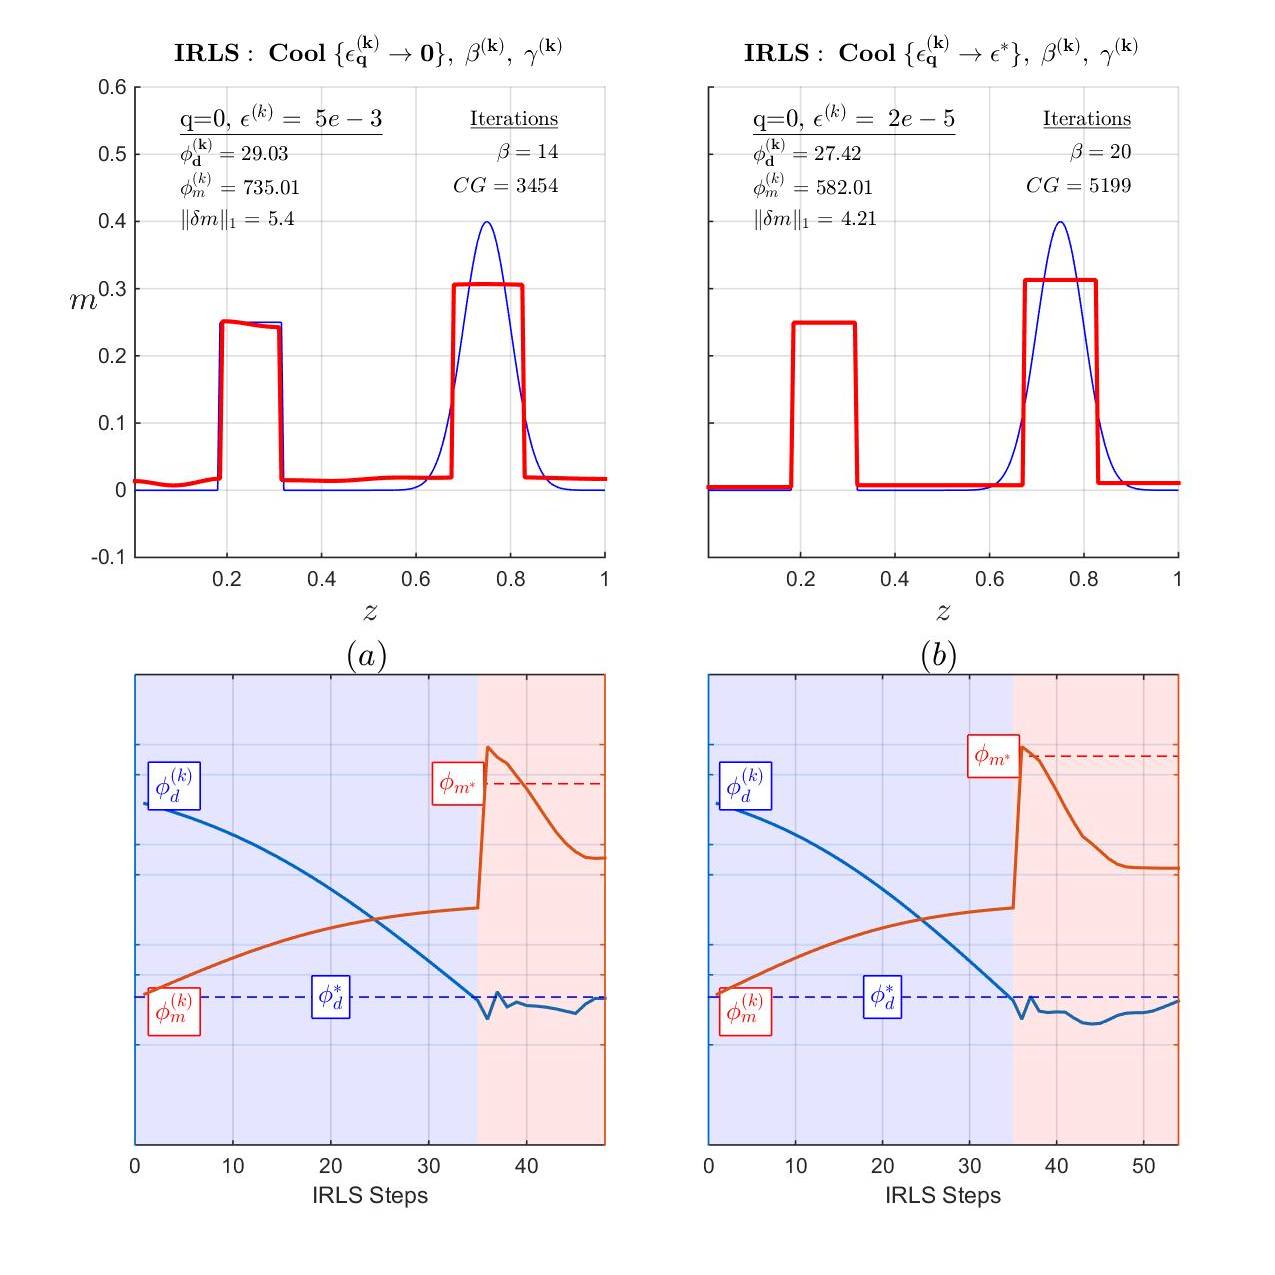
\includegraphics[scale=0.57]{1D_IRLS_algo3}
\caption{(Top) Recovered models from two different algorithms used to implement the IRLS method for $q=0$ with cooling of the threshold parameter $\epsilon$. (Bottom) Measure of model misfit and model norm as a function of iterations. Both algorithms adjust $\beta$ and scaling parameter $\gamma^{(k)}$ between each IRLS iteration. (a) In the first case, the threshold parameter $\epsilon$ is monotonically reduced until reaching the convergence criteria. The solution is sparser than the previous algorithm, even though $\epsilon$ is much larger than machine error.
(b) In the second case, $\epsilon$ is decreased until reaching the target threshold $\epsilon^*$. The solution is blocky, penalizing small model gradients.}
\label{fig:1D_IRLS_algo3}
\end{figure}

The method proposed above is advantageous as it does not require a specific choice of threshold parameters $\epsilon_p$ and $\epsilon_q$.
It does depend however on the specified convergence criteria $\delta \phi_m^{(k)}$.
In some cases, the algorithm may converge too quickly before reaching the desired level of sparsity. 
Alternatively, the algorithm may become overly expensive if the convergence criteria is too restrictive or the solution oscillates around the minimum. 
Secondly, the stabilizing parameter $\epsilon$ can be interpreted as an $effective\;zero$, penalizing specific ranges of model parameters.
It may therefore be necessary to determine a minimum threshold value in order to guarantee convergence and penalize the right model values.

Since the initialization of the IRLS requires a good approximation of the model via a least-squares solution, an estimate of the distribution of model parameters is available for analysis.
The value of an optimal $\epsilon^*$ can be chosen directly by the user based on $a\;priori$ information. Alternatively the choice can be based on the distribution of model values.
Figure~\ref{fig:1D_Model_curve}(a) presents the distribution of model and model gradients obtained from the smooth $l_2$-norm inversion.
Both curves display a sharp corner around which the model parameters rapidly change. 
Similarly, \cite{ZhdanovTolstaya2004} suggest an L-curve based on the change in model norm such that:
\begin{equation}\label{s_ms}
\begin{split}
s_{MS}(\epsilon) &= \mathbf{m^T R_\text{s}^T R_\text{s} m} \\
s_{MGS}(\epsilon) &= \mathbf{m^T G_\text{x}^T R_\text{x}^T R_\text{x} G_\text{x} m}\;,
\end{split}
\end{equation}
where the model norm $s_{MS}$ and model gradient norm $s_{MGS}$ are computed over a range of $\epsilon$ values as shown in \ref{fig:1D_Model_curve}(b). I found experimentally that both approaches were valid but did not always yield a well defined corner.
More research may be needed to determine the most robust approach.

As a final experiment, I invert the 1-D example using the point of maximum curvature on the $s_{MGS}$ curve as a minimum threshold  for the model gradients  ($\epsilon_q^*=2e-5$) . Figure~\ref{fig:1D_IRLS_algo3}(b) presents the model after convergence.
I note that the result is more blocky than the one previously obtained with the convergence criteria.
The inversion is, computationally, slightly more expensive due to the larger number of IRLS steps to reach the target threshold parameter $\epsilon_q^*$. 


\begin{figure}[p]
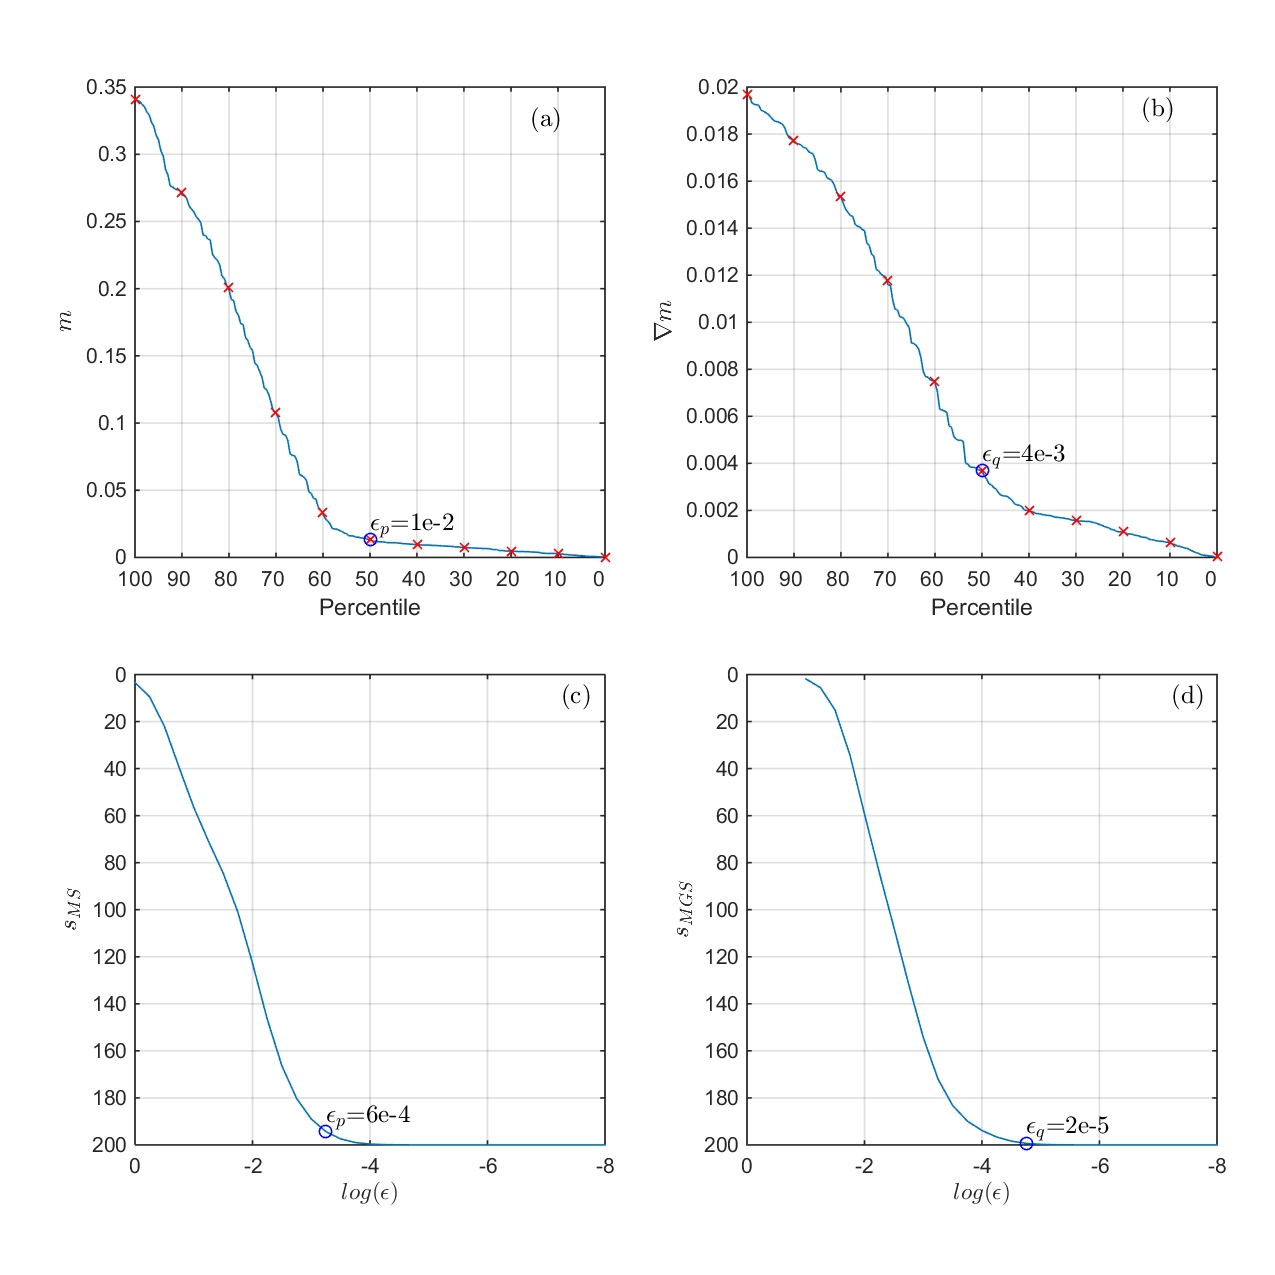
\includegraphics[scale=0.6]{1D_Model_curve}
\caption{(a) Distribution of model parameters and (b) model gradients recovered from the smooth $l_2$-norm regularization.
Both curves show a sharp corner around which the model functions vary rapidly. Similarly, a measure of (c) model norm $s_{MS}$ and (d)  model gradient norm $s_{MGS}$ can be computed over a range of $\epsilon$ values, yielding a similar $L-curve$. The point of maximum curvature can be used to determine the optimal $effective\;zero$ parameter $\epsilon_p$ and $\epsilon_q$. }
\label{fig:1D_Model_curve}
\end{figure}
%The S-IRLS algorithm can be summarized as follow:
%\begin{itemize}
%\setlength\itemsep{0em}
%\item{Phase l \textemdash $L_2$-norm initialization:} 
%\begin{itemize}
%	\setlength\itemsep{0em}	
%	\item Inversion with $l_2$-norm regularization $\rightarrow$ $\mathbf{m}^{(0)}$ , $\beta^{(0)}$
%	\item Set threshold values $\epsilon_p$, $\epsilon_q$ (see section \ref{eps_algo})
%\end{itemize}	
%\item Phase ll \textemdash S-IRLS iterations: $while \; \tau^{(k)} < 1\%$
%\begin{itemize}
%	\setlength\itemsep{0em}		
%	\item Generate IRLS weights: $\mathbf{R}_s$, $\mathbf{R}_x$
%	\item Compute gradient scales: $\eta_p$, $\eta_q$ $\rightarrow$ $\mathbf{\hat R}_s$, $\mathbf{\hat R}_x$
%	\item Compute regularization scaling: $\gamma^{(k)}$ 
%	\item Solve $\phi^{(k)}$: $\mathbf{m}^{(k)}$  $\rightarrow$ $\mathbf{m}^{(k+1)}$
%\end{itemize}
%\item Phase lll \textemdash Adjusting $\beta$: $while \; \phi_d^{(k)} \ne \phi_d^*$
%\begin{itemize}
%	\item Adjust trade-off parameter $\rightarrow$ $\beta^{(k)}$
%	\item Solve $\phi^{(k)}$: $\mathbf{m}^{(k)}$  $\rightarrow$ $\mathbf{m}^{(k+1)}$ 
%\end{itemize}
%\end{itemize}

%The S-IRLS method is non-linear with respect to the model parameter and requires several iterations before converging to stable solution.
%Just as for the Gauss-Newton steps, I need a criteria to stop the iteration process.
%During Phase ll of the algorithm, I monitor the change in distribution of model values such that :
%\begin{equation} \label{eq:dcdm}
%	\tau^{(k)} =  \frac{ | \xi^{(k)} -  \xi^{(k-1)} |}{\xi^{(k)}} \times 100
%\end{equation}
%where I define a clustering parameter $\xi$ as:
%\begin{equation}
%\begin{split}
%&\xi^{(k)} = \sum_{i=1}^M y_i  \\
%&\begin{cases} 
%y_i = 1 & if\; m_i < \epsilon \\
%y_i = 0 & if\; m_i \ge \epsilon
%\end{cases}
%\end{split}
%\end{equation}
%The clustering term $\xi$ simply measures the number of model values smaller than $\epsilon$.
%I found experimentally that monitoring the clustering of model parameters is a more robust measure of convergence than other measures such as used in Equation~\ref{Convergence}.
%For $p < 1$, only the smallest model parameters are penalized, and they may not have a big impact on the overall measure of $\|\mathbf{m}^{(k)}\|$, yet the model may still be changing around $\epsilon$. 
%Motoring the number of cells on either side of $\epsilon$ reveals if the inversion has reached a stable solution specifically for the model values targeted by the norm.  

%%%%%%%%%%%%%%%%%%%%%%%%%%%%%%%%%
\newpage
\section{Scaled-IRLS method (S-IRLS)}\label{S-IRLS}
The blocky solution found previously is expected from an $l_0$-norm penalty on the gradient. But it is clearly not appropriate to recover  the true synthetic model, which is both smooth and sparse.
Building upon the previous section, I explore different combinations of norms on the model and model gradients in order to $shape$ the penalty function. This function should allow any available $a\;priori$ information to be incorporated in the solution.
My first attempt uses an $l_0$-norm on the model combined with and $l_2$-norm on the model gradients, or $\{p=0 , q = 2\}$.
For this combination of norms, I would expect the solution to be both sparse and smooth, better approximating the width of the rectangular pulse and Gaussian anomaly.
Figure \ref{fig:1D_Eta_test}(a) shows the solution after convergence of the IRLS algorithm.
I here identify an important issue with the current IRLS method involving various norm measures within the same objective function. 
The solution is clearly dominated by the sparsity constraint. 
In this case, the $l_0$-norm penalty on the model suppresses the $l_2$-norm penalty on the model gradient, yielding a strictly sparse solution without smoothness constraint.

\begin{figure}[p]
\centering
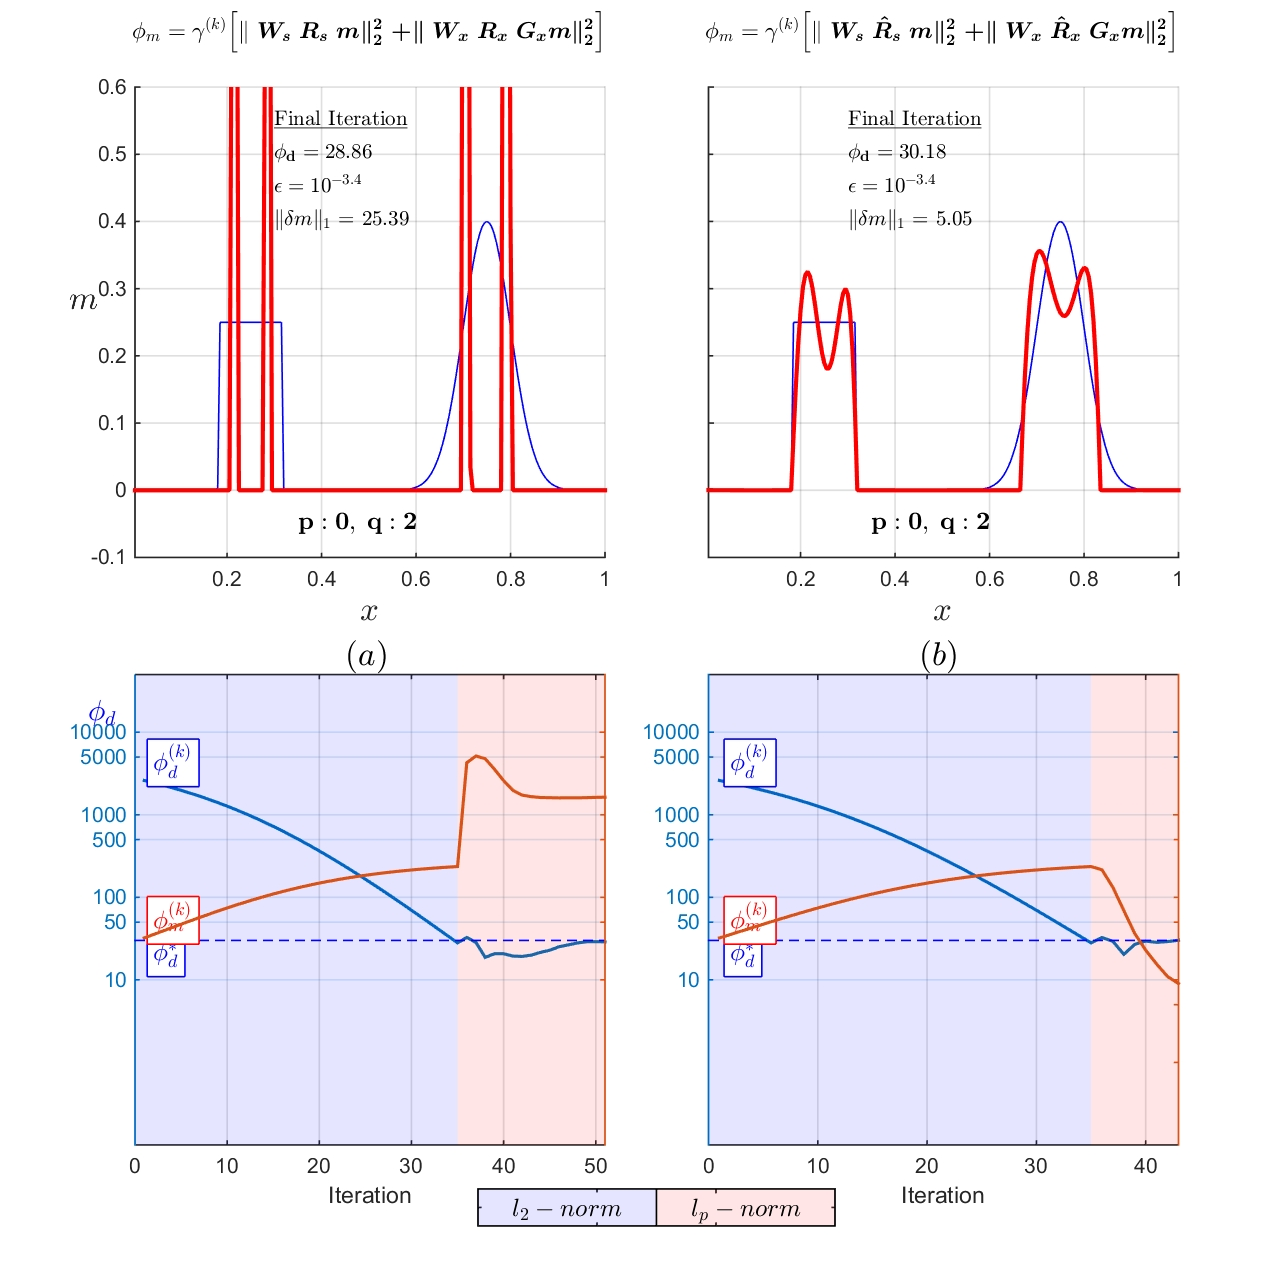
\includegraphics[scale=0.6]{1D_Eta_test}
\caption{(a) (Top) Recovered model using a mixed-norm regularization for $p=0$, $q=2$, $\epsilon=1e-3$. (Bottom) Measure of model misfit and model norm as a function of iterations. The inversion converges to a sparse solution without apparent penalty on the gradient, indicative of an imbalance in the regularization. (b) Recovered model and convergence curves after rescaling of the regularization, yielding a model that is both sparse and smooth as expected from the applied mixed-norm .}
\label{fig:1D_Eta_test}
\end{figure}

To understand the issue, it is useful to look at the linear system defined by \ref{eq:dphi_dm_lp}. 
Recall that a solution is found along the gradient of the objective function, which from \eqref{eq:dphi_dm} can be written explicitly as:
\begin{equation}\label{StepDirection}
\begin{split}
\frac{\partial \phi(m)}{\partial m} &= \big(\mathbf{F^T\;d} - \mathbf{F^T\;F\;m}\big) - \beta\big (\;  \mathbf{g_s}(m) + \mathbf{g_x}(m)\;\big ) \\
\mathbf{g_s}(m) &=  \mathbf{R_{\text{s}}^T}\; \mathbf{W_{\text{s}}^T} \mathbf{W}_s \;\mathbf{ R}_s\; \mathbf{m}\\
\mathbf{g_x}(m) &=  \mathbf{G_{\text{x}}^T} \;\mathbf{R^T}_x\; \mathbf{W_{\text{x}}^T}\mathbf{W}_x \;\mathbf{R}_x \; \mathbf{G}_x\; \mathbf{m} \;.
\end{split}
\end{equation}
I divided \eqref{StepDirection} into three parts to highlight the different components of the total gradient direction.
The first term $\big(\mathbf{F^T\;d} - \mathbf{F^T\;F\;m}\big)$ is related to the misfit function and depends solely on the ability of the model to reproduce the data $\mathbf{d}$. 
The second term $ \beta\big (\;  \mathbf{g_s}(m) + \mathbf{g_x}(m)\;\big )$ is related to the regularization function, which depends on the IRLS weights $\mathbf{R_s}$ and $\mathbf{R_x}$ computed in \ref{eq:R_w}.

To illustrate the importance of scaling between the function gradient terms I form a slightly different 2-variable problem where:
\begin{equation}
	\mathbf{F} = 
	\begin{bmatrix}
	0 & 1
	\end{bmatrix}\:,\:
	\mathbf{d} = 1 .
\end{equation}
Figure \ref{fig:IRLS_Phis_Phix}(a) displays contours along the surface formed by the $l_2$-norm measure of data residual $\|\mathbf{ F\;m - d }\|_2^2$, where this time the null-space of $\mathbf{F}$ lies parallel to the $x$-axis. 
I simplify the problem by having cell size and weights all equal to one so the objective function can be written as:
\begin{equation}\label{eq:Toy_phi}
\begin{split}
\phi(m) &= \phi_d + \beta \left[ \phi_s + \phi_x \right] \\
&= \|\mathbf{Fm - d}\|_2^2 + \beta \left [ {\| \mathbf{m}\|}^2_2 +  {\|  \mathbf{ G_\text{x} \; m}\|}^2_2  \right ] \;.
\end{split}
\end{equation}
By setting a small trade-off parameter ($\beta = 1e-3$), I can focus on the solution space along the null-space of \textbf{F} marked by the red dash line, as shown in Figure \ref{fig:IRLS_Phis_Phix}(e).
The global minimum of the objective function lies at $\mathbf{m} = [0.5;1]$, where the partial gradients of $\frac{\partial\phi_s}{\partial\;m_1}$ and $\frac{\partial\phi_x}{\partial\;m_1}$ have equal and opposite signs.
Here the two regularization functions use an $l_2$-norm measure, hence the optimal solution is at mid-distance from their respective minimums.
This simple example shows that the actual value of the individual norms do not matter, but rather the relative magnitude of the gradients along the  minimum of $\phi_d$.

\begin{figure}[h!]
\centering
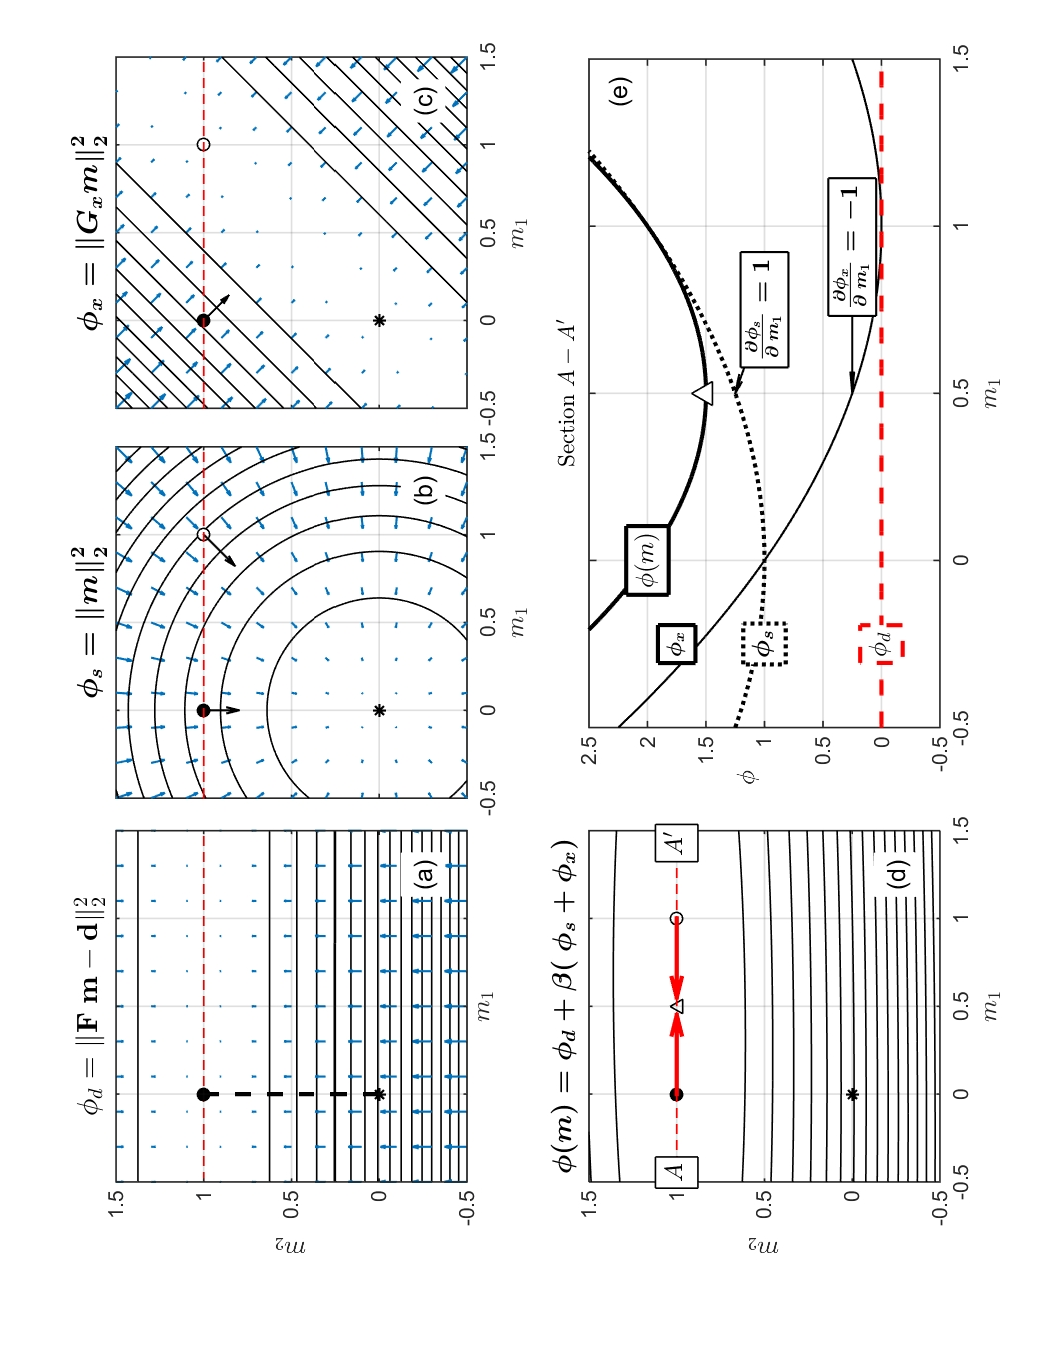
\includegraphics[scale=0.55, angle=270]{IRLS_toy_Phis_Phix}
\caption{Contour maps for (a) the misfit function $\phi_d$, (b) the model norm $\phi_s$ and (c) the norm of model gradients $\phi_x$. (d) The total objective function $\phi(m)$ has a global minimum located at $\mathbf{m}=(0.5,1.0)$ for a given small trade-off parameter ($\beta = 1e-3$). The direction of update is shown for two starting models $\mathbf{m}^{(0)}$ (black and white dot). (e) Section through the objective function along the minimum of $\phi_d$. The global minimum occurs where the partial gradients of $\frac{\partial\phi_s}{\partial\;m_1}$ and $\frac{\partial\phi_x}{\partial\;m_1}$ have equal and opposite signs.}
\label{fig:IRLS_Phis_Phix}
\end{figure}

The behavior of the $l_0$-norm for small $p$ and $\epsilon$ values can easily explain the result obtain in Figure~\ref{fig:1D_Eta_test}(a).
Figure~\ref{fig:Lp_g_scaled}(a) compares the function gradients for different norm penalties as a function of $p$ values. 
In this case, the function gradients $\mathbf{g_s}$ measured with the $l_0$-norm are always much larger than the function gradients $\mathbf{g_x}$ measured with the $l_2$-norm, except at $m_i = \{0, \sqrt{1-\epsilon^2}\}$.
The solution can therefore only be sparse with few non-zero model values required to satisfy $\phi_d^*$. 
The penalty on model gradients had no influence on the solution.

Just as I added the parameter $\gamma^{(k)}$ to balance the relative importance between the misfit function and the regularization, I also want to control the relative scaling between the various regularization functions in terms of their gradients.
In other words, I want to find a scaling parameter that makes the gradient of any $l_p$-norm function to intersect, elsewhere than at $m_i = \{0, \sqrt{1-\epsilon^2}\}$.

I here introduce a scaling parameter $\eta$:
\begin{equation} \label{eq:eta}
\eta =  \epsilon^{(1-p/2)} \;,
\end{equation}
where once again $p$ denotes the $l_p$-norm penalty and $\epsilon$ is a small value used to approximate the norm.
Adding the scaling parameter $\eta$ to \ref{eq:dphidm}, the partial gradients of the objective function  become:
\begin{equation} \label{S-lp_dphidm}
\frac{\partial \phi_m}{\partial m} = \;\frac{\epsilon^{(1-p/2)}  x_i}{{{(x_i}^{2} + \epsilon^2 )}^{1-p/2}}  \;.
\end{equation}

\begin{figure}[h!]
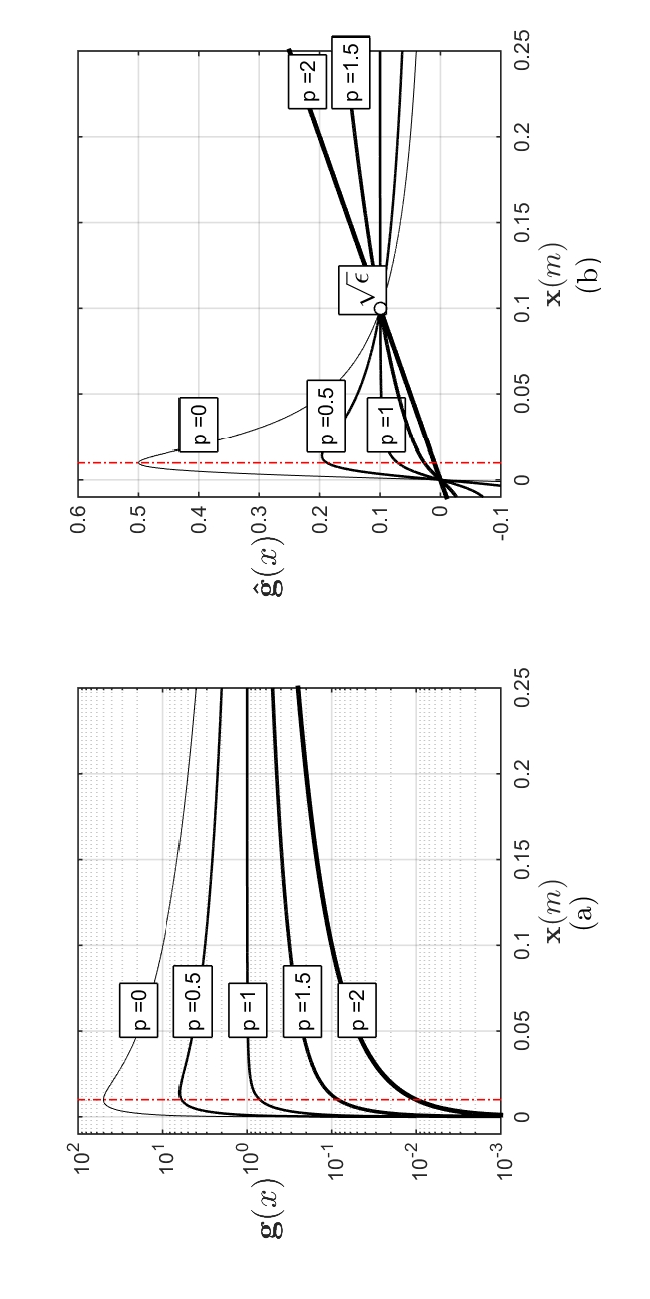
\includegraphics[scale=0.58,angle=270]{Lp_g_scaled}
\caption{(a) Partial gradients of approximated $l_p$-norm penalties for a fix stabilizing parameter $\epsilon =1e-2$. Gradients for $p < 1$ are consistently larger on the interval $[0 < x_i < \sqrt{1-\epsilon^2}]$, making it hard to combine multiple norm penalties within the same objective function. (b) Function gradients after applying a scale of $\epsilon^{(1-p/2)}$, forcing each $l_p$-norm to intersect at $m = \sqrt{\epsilon}$.   }
\label{fig:Lp_g_scaled}
\end{figure}

Looking at the gradient for $x_i=\sqrt{\epsilon}$, \ref{S-lp_dphidm} simplifies to:
\begin{equation*}
\frac{\partial \phi_m}{\partial m} = \;\frac{\epsilon^{1/2}}{{(1+ \epsilon )}^{1-p/2}} \;.
\end{equation*}
Then assuming that $\epsilon \ll 1$:
\begin{equation} \label{approx_lp}
\frac{\partial \phi_m}{\partial m}\approx \; \epsilon^{1/2} \;.
\end{equation}
Hence after applying the scaling $\eta$, the gradient of the $l_p$-norm is independent of the $p$-value exactly at $m=\sqrt{\epsilon}$, and has also a gradient $\frac{\partial \phi}{\partial m}=\sqrt{\epsilon}$, as shown in Figure~\ref{fig:Lp_r_dphidm}(c).
Therefore, $\sqrt{\epsilon}$ is a critical point around which all norm penalties can influence the solution.
In this manner, two penalty functions with different $p$-values can coexist within a regularization function and achieve different objectives.
 
 Adding this final scaling to \ref{eq:scaled_Lp_phi} yields a \emph{Scaled Iterative Re-weighted Least Squares} (S-IRLS) regularization function such that: 
\begin{equation} \label{eq:S-IRLS}
\hat \phi_m^{(k)} = \gamma^{(k)} \Big ( {\| \mathbf{W_\text{s} \; \hat R_\text{s} \; m}\|}^2_2 +  {\|  \mathbf{ W_\text{x}\; \hat R_\text{x} \; G_\text{x} \; m}\|}^2_2  \Big ) \;.
 \end{equation}
I define a Scaled-IRLS weighting matrix $\mathbf{\hat R}$ such that:
\begin{equation} \label{eq:eta}
\begin{split}
{\hat R}_{s_{ii}}  &= \sqrt{\eta_p}{\Big[ {({m_i}^{(k-1)})}^{2} + \epsilon_p^2 \Big]}^{(p/2 - 1)/2} \\
{\hat R}_{x_{ii}}  &= \sqrt{\eta_q}{\Big[ {\left ({\frac{\partial m_i^{(k-1)} }{\partial x}}\right)}^{2} + \epsilon_q^2 \Big]}^{(q/2 - 1)/2}  \\
\eta_p &=  {\epsilon_p}^{(1-p/2)} \\
\eta_q &=   {\epsilon_q}^{(1-q/2)}  \;, 
\end{split}
\end{equation}
where $\epsilon_p$ and $\epsilon_q$ are the stabilizing parameters for the $l_p$-norm of the model and model gradients respectively.
Note that for $p=2$, the scaling parameters $\eta$ is equal to one, hence we recover the the classic $l_2$-norm regularization. 

 Figure \ref{fig:1D_Eta_test}(b) presents the result after a re-scaling of the gradient descent. 
Both the $l_0$-norm penalty on the model and the $l_2$-norm penalty on the model gradients are represented, yielding a solution that is both sparse and smooth. 
I now have a flexible and robust regularization function. This allows us to explore a wide range of solutions, or $l_p$-space of solutions, combining various norms on the model and model gradients.

\subsection{Cell-based weights (${w}_r,\; w_m$)}\label{Wr_Section}
In \cite{LiOldenburg1996}, a depth weighting function is added to counter the natural decay of potential fields. 
The rapid decay in sensitivity is an important problem in geophysics as most data sets are acquired from the surface.
The same idea can be used to incorporate any \emph{a priori} information regarding the spatial distribution of model parameters.
In this section, I investigate the effect of having such cell-based weighting applied directly to the sensitivity matrix, compared to having it applied to the regularization function as previously formulated in \ref{eq:Phi_disc} .

Following the weighted sensitivity formulation of \cite{LiOldenburg1996}, the objective function with S-IRLS regularization takes the form:
\begin{equation} \label{eq:phi_Wrm}
 \phi(\hat m) = \|\mathbf{W_d \;(\hat F\; \hat m - d)}\|_2^{2} + \gamma^{(k)} \Big [ {\|\mathbf{W_\text{s}  \;\hat R_\text{s} \; \hat m}\|}^2_2  +   {\|\mathbf{  W_\text{x}  \;\hat R_\text{x} \; G_\text{x} \; \hat m}\|}^2_2  \Big ] \;,
 \end{equation}
 where:
\begin{equation*}
\begin{split}
\mathbf{\hat F} &= \mathbf{F\;W_\text{r}^{-1}} \\
\mathbf{\hat m} &= \mathbf{W_\text{r}\;m} \\
\mathbf{W_\text{r}} &= diag \left( e^{j\: z / (2 \pi)} \right )\;,
\end{split}
\end{equation*}
where the matrix $\mathbf{W_\text{r}}$ hold the inverse exponential describing the decay of the kernel functions presented in \ref{eq:kernel_1D}.  
Similar sensitivity based weighting is used in the \textit{Minimum Support} functional of \cite{PortniaguineZhdanov02}.

Using both formulations, I invert the same 1-D example presented in Figure\ref{fig:1D_IRLS_algo3} and \ref{fig:1D_Eta_test}.
In the first experiment, I apply a sparsity constraint on the model gradients for $q=0, \alpha_s =0$. 
Figure \ref{fig:1D_Wr_in_vs_out}(a) compares the true and recovered models after convergence.
I observe the solution obtained with the $\phi({\hat m})$ formulation is skewed in the direction of the sensitivity weighting.
Similarly, Figure \ref{fig:1D_Wr_in_vs_out}(b) shows the recovered model for the combination of $p= 0,\;q=2$.
While the recovered anomaly over the rectangular pulse is both smooth and sparse, I note that the solution tends to favor a strictly sparse model further at depth over the Gaussian function.
On the other end, the solution obtained with the $\phi({m})$ formulation remains smooth and sparse over both anomalies equally.

Issues encountered with the $\phi({\hat m})$ formulation are due to the IRLS weights computed in \ref{eq:Rs_Rx}.
Written explicitly in terms of weighted model parameters, the linearized IRLS norm from \ref{eq:IRLS_phi} can be written as:
\begin{equation}\label{Weighted_IRLS}
\phi_{\hat m}^{(k)} =  \sum^{nc}_{i=1} \frac{{(w_i x_i)}^2}{ {\left[{(w_i x_i^{(k-1)})}^2 + \epsilon^2 \right ]}^{1-p/2}} \;.
\end{equation}
Factoring out the cell-based weight $w_i$, equation~\ref{Weighted_IRLS} becomes:
\begin{equation}\label{Weighted_IRLS_Facto}
\phi_{\hat m}^{(k)} =  \sum^{nc}_{i=1}  \frac{w_i^p x_i^2}{ {\left[{(x_i^{(k-1)})}^2 + \epsilon^2/w_i^2 \right ]}^{1-p/2}} \;.
\end{equation}
The important point to note is that the weights are now function of the $p$-value, while the threshold parameter $\epsilon$ depends on the cell-based weights.
In most cases, the sensitivity weights increase with distance from the observation location, which in turn reduce the threshold parameter $\epsilon$ and increase the influence of sparse norms.
This explains the increase in sparsity constraint with distance as observed in Figure~\ref{fig:1D_Wr_in_vs_out}.
In order to preserve the character of cell-based weights, it is important to isolate their effect from the $l_p$-norm penalty.
The same idea extends to any type of cell-based weights (i.e. volumetric, \emph{a priori}).
In the following chapter, various norm measures will be used simultaneously on the model and model gradient.
The predictability and stability of the algorithm depends greatly on the scaling between the various components of the objective function.

\begin{figure}[h!]
\centering
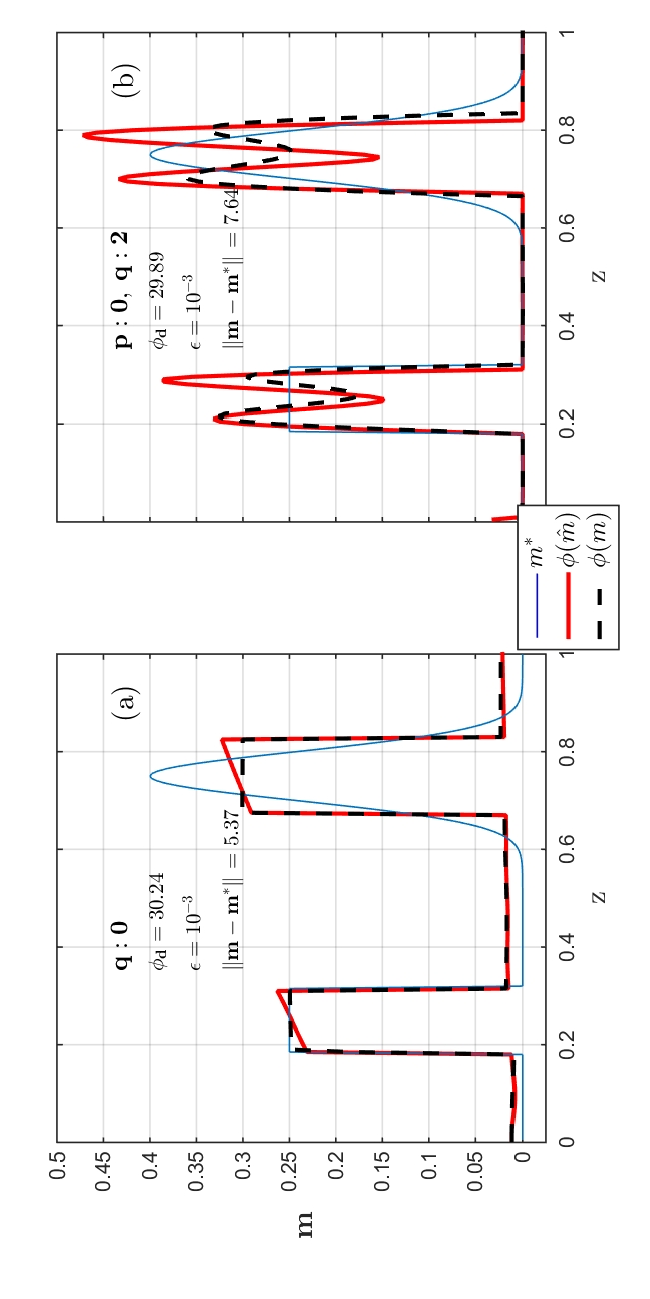
\includegraphics[scale=0.55, angle=270]{1D_Wr_in_vs_out}
\caption{Recovered models for two different depth weighting  formulations: (red)  weighted sensitivity $\phi(\hat m)$,  (black)  weighted regularization $\phi(m)$.
(a) True and recovered models using the $\phi(\hat m)$ and $\phi(m)$ formulations for penalty applied on the model gradients for $q=0$ and (b) for $p= 0,\;q=2$.
The weighted sensitivity formulation $\phi(\hat m)$ increases the influence the regularization function with distance along the $x$-axis, skewing the model towards the right.}
\label{fig:1D_Wr_in_vs_out}
\end{figure}

\newpage
%%%%%%%%%%%%%%%%%%%%%%%%%%%%%%%%%%%%%%%%%%%%%%%%%%
\section{Mixed $l_p$-norm regularization}
I showcase the robustness and flexibility of the S-IRLS algorithm by inverting a total of 441 models, corresponding to all the combinations of norms on the interval $0 \leq p \leq 2$ and $0 \leq q \leq 2$, on a 0.1 increment.
Figure \ref{fig:1D_Results_ALL}(a) presents a contour map of the final model errors $\|\delta\mathbf{m}\|_1$ recovered after each inversion.
The gradual variation in model error is a good indicator of the predictability of the algorithm, as small changes in the regularization yield equivalently small changes in the solution.
For each inversion, the trade-off parameter $\beta$ was adjusted to fit within $\pm 2\%$ of the target data misfit for appropriate comparison of the results, as shown in \ref{fig:1D_Results_ALL}(b). 
In this case, the optimal model is found with a combined norm of  [$p=1.5$,  $q=0.4$]. 
In this particular case, the worst recovery was obtained with $p=0,\; q=2$, yielding a sparse solution with few large oscillations.
Even though this type of analysis would be computationally prohibitive for large scale inverse problems, it illustrates the flexibility of the S-IRLS method in designing an objective function reflecting specific characteristics. 

Nine of the inverted models are shown in Figure \ref{fig:1D_Results} for comparison. 
As expected from the property of the IRLS functions, small norms on the gradient promote blocky solutions. From right to left, the inversion result tends to favor right-angled anomalies. From bottom to top, smaller norms on the model parameter enforce sparse solutions with few non-zero values.

\begin{figure}[p]
\centering
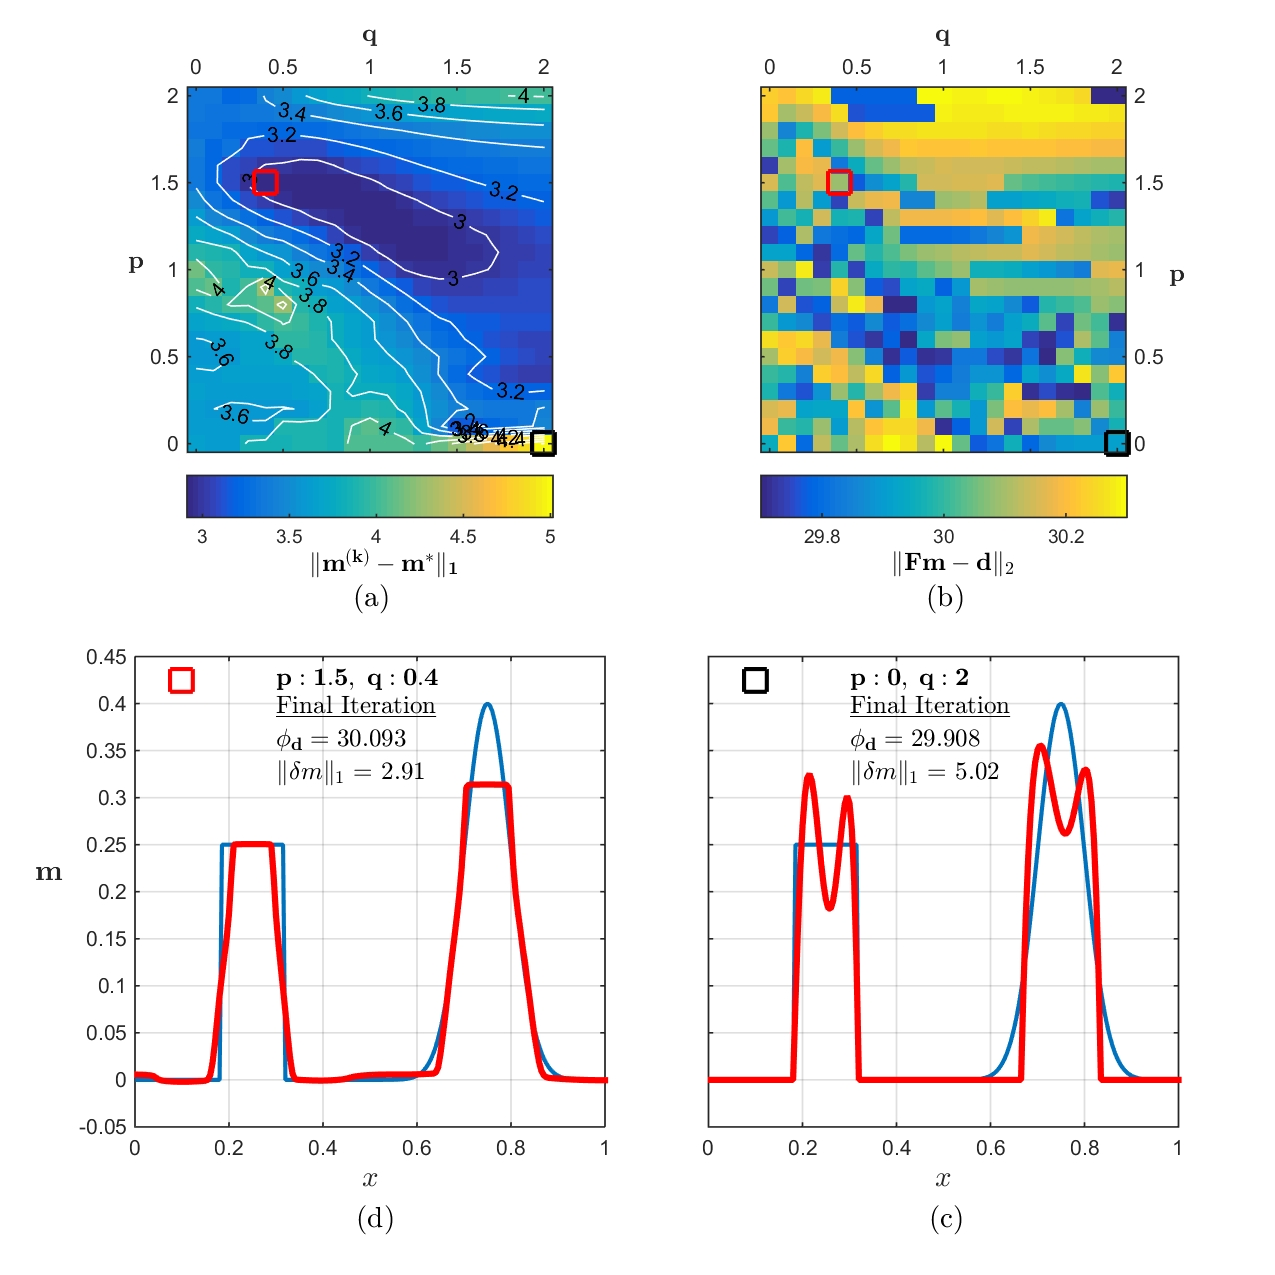
\includegraphics[scale=0.62]{1D_Results_ALL}
\caption{(a) Model error $\| m - m{*}\|_1$ and (b) misfit function for the 441 inverted models using a range of regularization with mixed-norm penalty on the model for $0 \leq p \leq 2$ and on model gradients for $0 \leq q \leq 2$. (c) The largest model error ($\| \delta \mathbf{m}\|_1$) was obtained with the mixed-norm for $p=0,\;q=2$, compared to (d) the optimal solution found with $p=1.5$ and $q=0.4$.}
\label{fig:1D_Results_ALL}
\end{figure}

\begin{figure}[t]
\centering
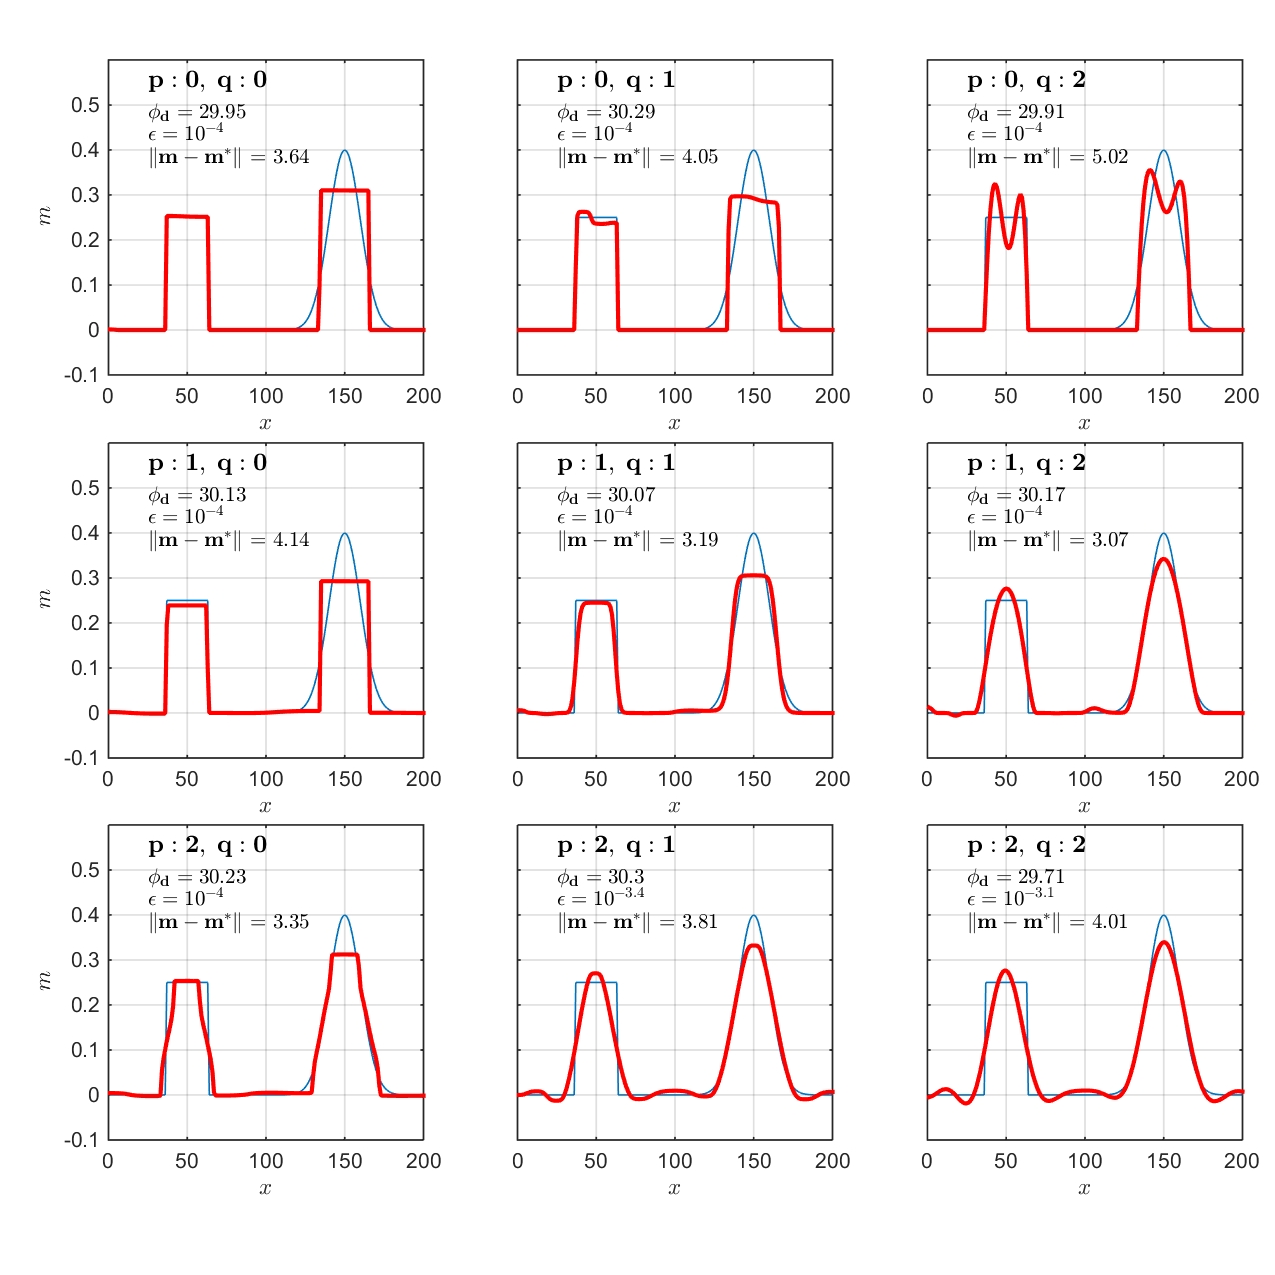
\includegraphics[scale=0.6, trim= 0.5cm 0 0 0]{1D_Results}
\caption{(a) Nine of the 441 inverted models for a range of mixed-norm penalties on the model and its gradient for $0 \leq p \leq 2$ and $0 \leq q \leq 2$. }
\label{fig:1D_Results}
\end{figure}

%%%%%%%
\subsection{Localized S-IRLS}\label{Localized_lp}
While I have so far implemented global regularization functions applied on the entire model, the S-IRLS method can easily be extended to problems made up of several sub-regions with varying norm penalties. Also based on the IRLS method, \cite{SunLi14} introduce an automated process to extract structural information from the data and impose either an $l_1$ or $l_2$-norm penalties to specific regions of the model.  
While designing this objective function can be challenging and may still require direct input from the user, their approach has great value as it increases the flexibility over traditional global penalty functions. 
The S-IRLS formulation has the potential to further generalize the work of \cite{SunLi14} in allowing the use of any norm penalty in the range of $0 \leq p \leq 2$. 

Suppose an N-dimensional model space $\mathbf{m} \in \Omega$, divided in $J$ sub-regions such that:
\begin{equation*}\label{eq:Subsets}
\begin{split}
	\mathbb{S} & = \{S_1, S_2, ... , S_J \;\Big| \;S_j \subset \Omega\ \;,\; j = 1,...,J\} \\
	S_i \cap S_j &=  \{\emptyset \;\Big| \;i,j = 1,...,J \;,\; j \neq i\}\;.
\end{split}
\end{equation*}
I can define a $model$ of $l_p$-norms by the union of each sub-domain:
\begin{equation}\label{p_vector}
\mathbf{p} = \bigcup_{j=1}^J S_j\;p_j\;,
\end{equation}
where the scaler $p_j$ defines the $l_p$-norm to be applied to the $j^{th}$ region of the model domain. 
Each sub-domain $S_j$ can have a distinct value for $p$ and $q$, penalizing the model values and model gradient differently than neighboring domains.
The transition in $l_p$-norm penalty can be smoothed after applying a linear transition across neighboring domains as defined by:
\begin{equation}\label{smooth_p_vector}
\begin{split}
\mathbf{\tilde p} &= \mathbf{A\;p} \\
\mathbf{A} &= 
		\begin{bmatrix}
			1/2 		& 		1/2	&  	0		& \dots  		&  0 \\
			\vdots	&  		 \ddots	&  	&   &  0\\
			0 		& 	\dots		& 		0	& 1/2 &  1/2 
		 \end{bmatrix} \;,
		 \end{split}
\end{equation}
where the transition between $l_p$-norm is extended over several cells by applying the averaging operator $\mathbf{A}$.
Allowing for multiple sub-domains requires only a slight change to the S-IRLS method presented in Section~\ref{S-IRLS}.
The general objective function for a 3-D discretized problem becomes:
 \begin{equation} \label{eq:Phi_IRLS}
\phi(m) =  \phi_d + \beta \gamma^{(k)} \Big [ {\| \mathbf{W}_s\;  \mathbf{\hat R}_s \;( \mathbf{m - m^{ref}})\|}^2_2  + \sum_{i = x,y,z}  {\|   \mathbf{W}_i \;  \mathbf{\hat R}_i  \; \mathbf{G}_i \; \mathbf{m}\|}^2_2  \Big ]\;,
\end{equation}
 such that the S-IRLS weights for the model and model gradients become:
\begin{equation}
\begin{split}
{\hat R}_{s_{ii}}  &= \sqrt{\tilde \eta_{p_i}}{\Big[ {({m_i}^{(k-1)})}^{2} + \epsilon^2_{p} \Big]}^{({\tilde p_i}/2 - 1)/2} \\
{\hat R}_{x_{ii}}  &= \sqrt{\tilde \eta_{q_{xi}}}{\Big[ {\left ({\frac{\partial m_i^{(k-1)} }{\partial x}}\right)}^{2} + \epsilon_q^2 \Big]}^{({\tilde q_{xi}}/2 - 1)/2}  \\
{\hat R}_{y_{ii}}  &= \sqrt{\tilde \eta_{q_{yi}}}{\Big[ {\left ({\frac{\partial m_i^{(k-1)} }{\partial y}}\right)}^{2} + \epsilon_q^2 \Big]}^{({\tilde q_{yi}}/2 - 1)/2}  \\
{\hat R}_{z_{ii}}  &= \sqrt{\tilde \eta_{q_{zi}}}{\Big[ {\left ({\frac{\partial m_i^{(k-1)} }{\partial z}}\right)}^{2} + \epsilon_q^2 \Big]}^{({\tilde q_{zi}}/2 - 1)/2}  \;.
 \end{split}
\end{equation}
Figure \ref{fig:1D_Mixed_norm} presents an optimal solution for the 1D problem, where I divide the model space into two regions.
The left half uses a $p=0, q=0$, whereas the right half imposes a $p=1$ and $q=2$.
The mixed-norm penalty function enforces the right characteristic to each portion of the model. 
The inversion recovers a sparse and blocky model over the rectangular pulse while at the same time managing to model the smooth Gaussian anomaly.
Consequently, the model error $\|\delta m\|$ is much smaller than any of the previous attempts.
The algorithm converges smoothly and rapidly to a stable solution.

\begin{figure}[t]
\centering
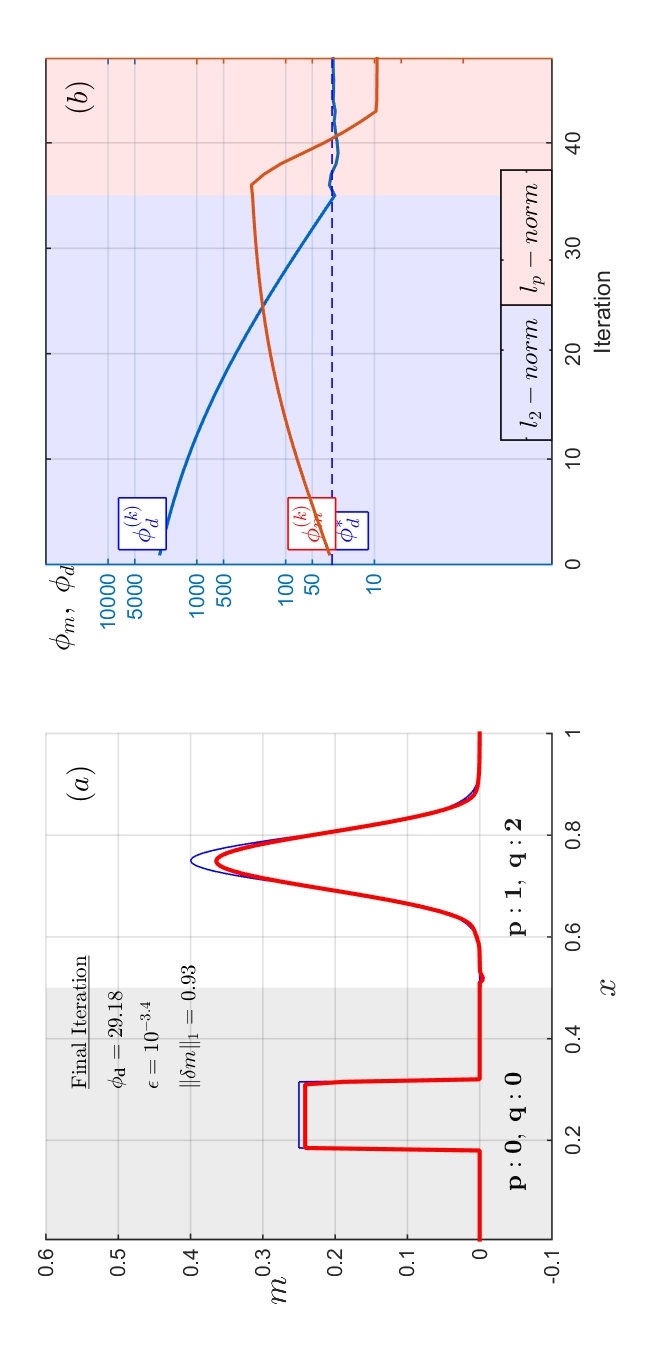
\includegraphics[scale=0.56, angle=270]{1D_Mixed_norm}
\caption{(Left) Improved solution for the 1-D problem after applying a localized mixed-norm penalty, where the regularization is divided into two regions with independent $l_p$-norm regularization: (left) $p = q = 0$, (right) $p=1 , q=2$. (Right) Convergence curves for the mixed-norm S-IRLS inversion.}
\label{fig:1D_Mixed_norm}
\end{figure}

\newpage
\subsection{2-D example}\label{2D_Section}
I test the S-IRLS algorithm on a 2-D synthetic model to further demonstrate the flexibility and robustness of the mixed-norm regularization. Analogous to the 1-D problem, the 2-D model consists of a square block and a smooth Gaussian anomaly, only this time the observations stations are located on both sides of the model domain. 
The kernel functions are exponentially decaying cosine functions of the form:
\begin{equation}
 	e^{-\omega\:r}\cdot sin(2 \pi \omega  r)\;,
\end{equation}
as shown in Figure \ref{fig:2D_Model_Kernel_data}. 

\begin{figure}[p]
\centering
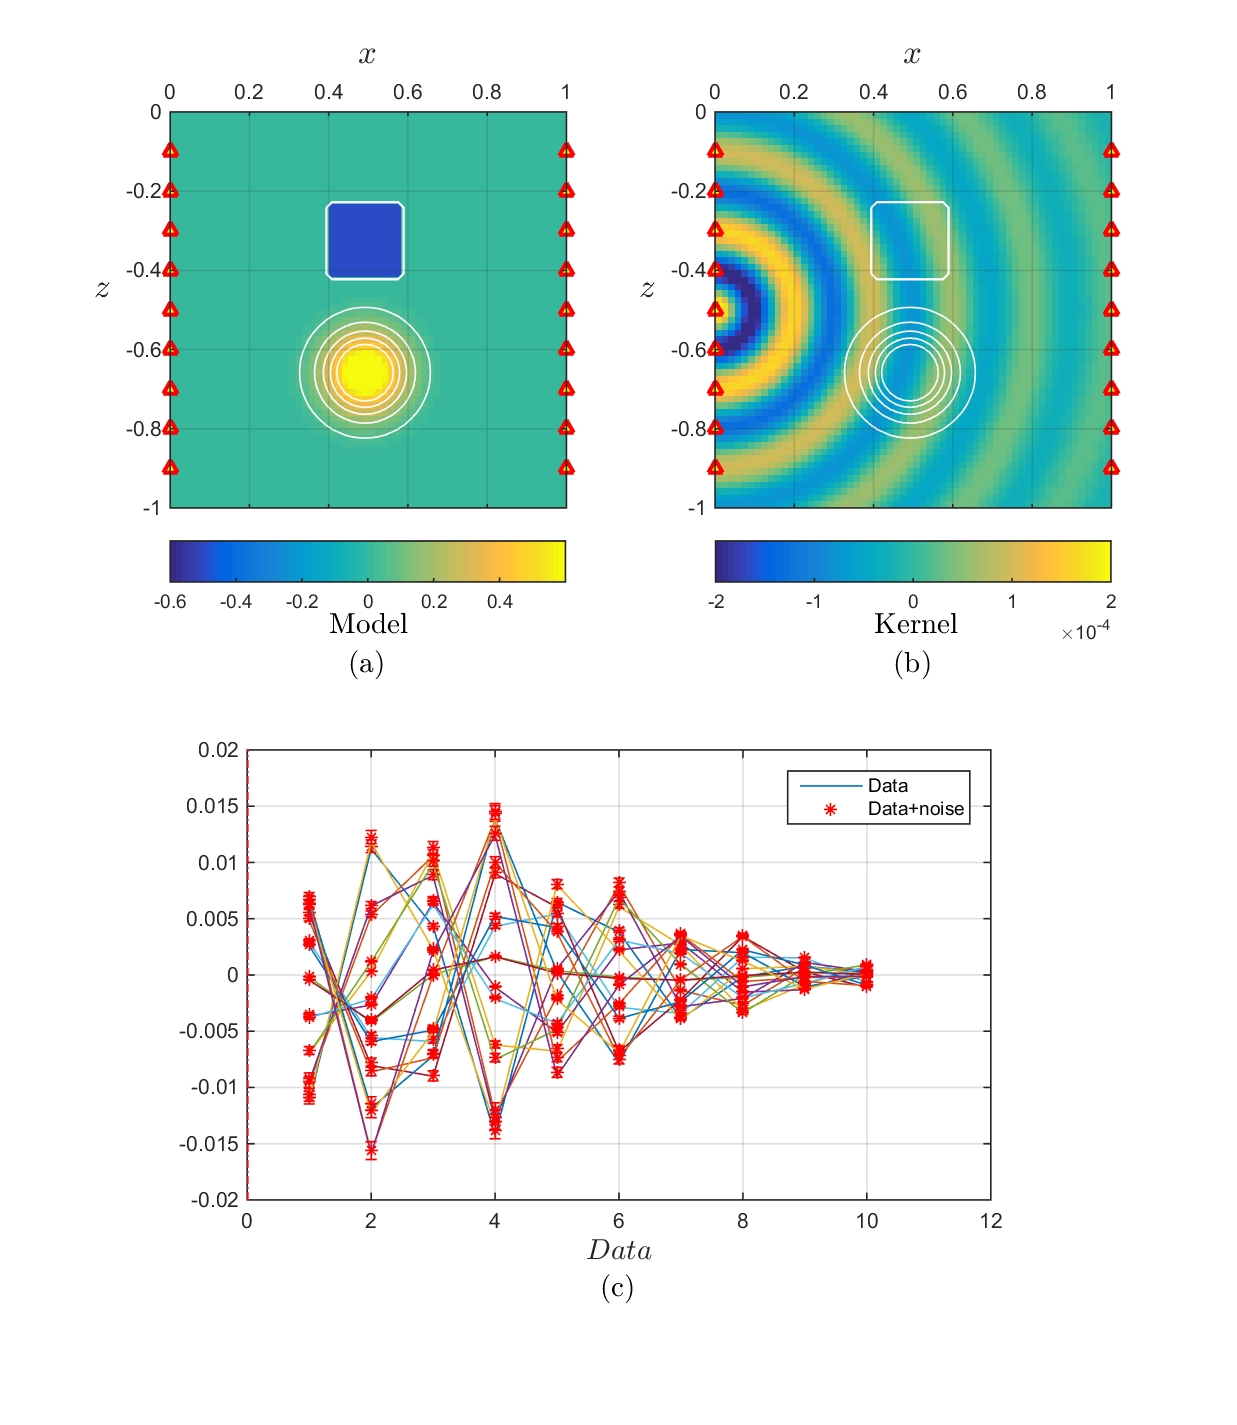
\includegraphics[scale=0.60]{2D_Model_Kernel_data}
\caption{(a) Synthetic 2-D model made up of a square block and a smooth Gaussian function. (b) Example of a kernel function for $e^{-\omega\:r}\cdot cos(2 \pi \omega  r)$ and (c) data generated from $\mathbf{d =F \; m}$. Five percent random  Gaussian noise is added. }
\label{fig:2D_Model_Kernel_data}
\end{figure}

Since we are now dealing with a 2-D problem, the regularization function involves a measure of model gradients in the $x$ and $z$-direction.
Most methods proposed in the literature, and presented in \ref{1D_Grad}, involve computing gradients with finite difference operators in orthogonal directions such that:
\begin{equation}\label{eq:grad}
\begin{split}
 	\frac{\partial m_i}{\partial x} &= \frac{m_{(i,j)} - m_{(i-1,j)}}{dx_{(i)}} \\
 	\frac{\partial m_i}{\partial z}  &= \frac{m_{(i,j)} - m_{(i,j-1)}}{dz_{(j)}}\;,
 	\end{split}
\end{equation}
where the indexes $(i,j)$ represent the cells ordering in the $x$ and $y$-direction respectively.
A second option is to penalize the absolute model gradients such that:
\begin{equation}\label{eq:mag_grad}
\begin{split}
	\nabla {m}_i  =  {\Big[ \big(\frac{\partial m_i^{(k-1)} }{\partial x}\big)^2 + \big(\frac{\partial m_i^{(k-1)} }{\partial z} \big)^2 \Big] }^{1/2}\;.
\end{split}
\end{equation}
The IRLS weights then become:
 \begin{equation}
 \begin{split}
 {\hat R}_{x_{ii}}  &= \sqrt{\tilde \eta_{q_{xi}}}{\Big[ {\left ({\nabla m_i}\right)}^{2} + \epsilon_q^2 \Big]}^{({\tilde q_{xi}}/2 - 1)/2}  \\
{\hat R}_{z_{ii}}  &= \sqrt{\tilde \eta_{q_{zi}}}{\Big[ {\left ({\nabla m_i}\right)}^{2} + \epsilon_q^2 \Big]}^{({\tilde q_{zi}}/2 - 1)/2}  \;.
   \end{split}
\end{equation}
%or
% \begin{equation}
%	\mathbf{r}_q^{(k)}  ={\Big( {(\mathbf{\nabla m}^{(k-1)})}^{2} + \epsilon^2 \Big)}^{\mathbf{q}/2 - 1} 
%\end{equation}
The same idea can easily be extended to three dimensions.
I illustrate the difference between both measures of model gradients on this 2-D problem. Figure \ref{fig:2D_Model_Grad_Test}(a) presents the recovered model using an $l_1$-norm penalty on the model gradients from the finite difference formulation. This yields blocky right-angled anomalies. Alternatively, penalizing the absolute model gradients from \eqref{eq:mag_grad}  allows for smooth corners as shown in \ref{fig:2D_Model_Grad_Test}(b). Both methods are valuable as they promote different solutions, which in some cases may better reflect the geometry of the true model. 

To accommodate both the blocky and the smooth anomaly, I divide the model space into three zones.
Figure \ref{fig:2D_Mix_lp_norms} presents the different $l_p$-norm zones defined over the two anomalies.
I extend the procedure of sub-regions presented in Section~\ref{Localized_lp} to this 2-D problem.
I impose sparse model values with the $l_1$-norm over the background region in order to get a simple model.
The norm on model gradient is variable and reflects the expected characteristics of the true model.   
I purposefully chose regions larger than the extent of the known anomalies in order to simulate a choice that could be made for a blind inversion. The goal is also to see if the transition from an $l_2$-norm to a $l_0$-norm can be done smoothly without creating artifacts.
Figure \ref{fig:2D_Mix_norm_result}(a) and (b) presents the recovered model after Phase l and Phase lll of the S-IRLS algorithm previously introduced in Table~\ref{tbl:IRLS_v4}.
Both models fit the data within 2\% of the target misfit $\phi_d^*$
The final mixed-norm model nicely recovers the blocky and smooth Gaussian anomaly. The transitions between the different $l_p$-regions appear to be seamless.

\begin{figure}[h]
\centering
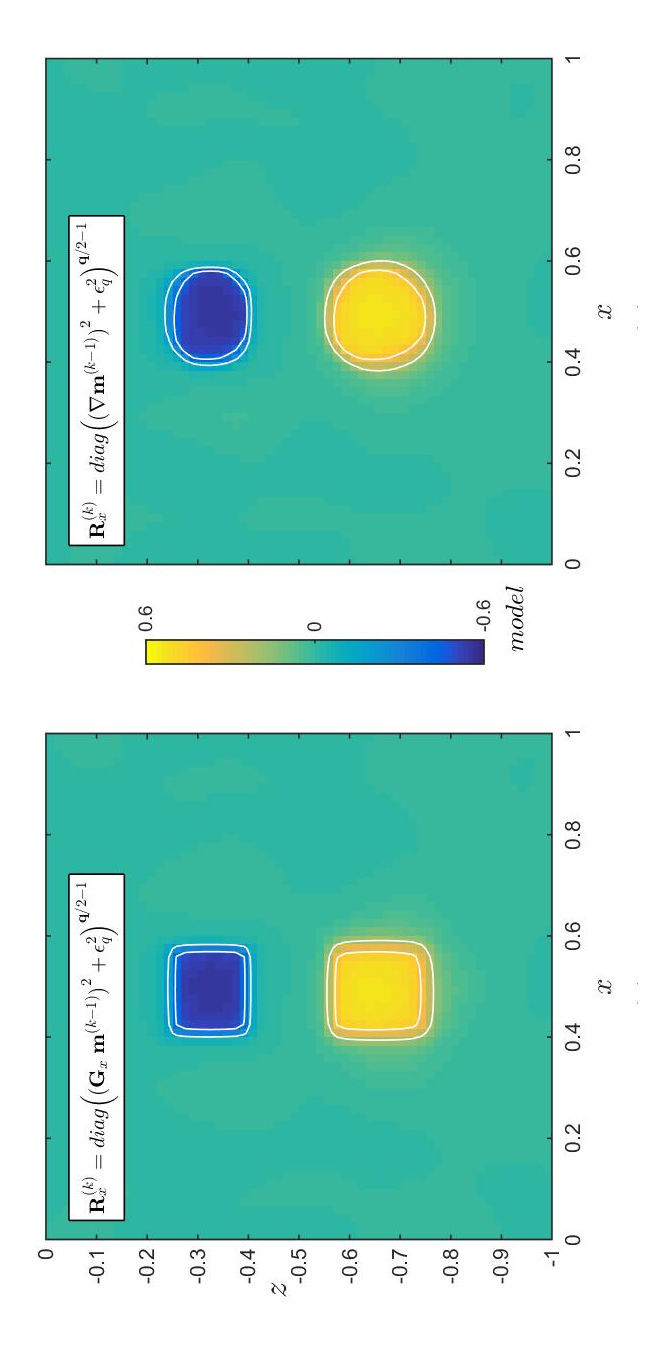
\includegraphics[scale=0.55, angle=270]{2D_Model_Grad_Test}
\caption{(a) Recovered model for $p = q_x = q_z = 1$ penalizing finite difference gradients in orthogonal directions, yielding right-angled anomalies. (b) Recovered model for the same norms but penalizing the absolute gradient of the model ($|\nabla \mathbf{m}|$) recovering round edges.}
\label{fig:2D_Model_Grad_Test}
\end{figure}

\begin{figure}[h!]
\centering
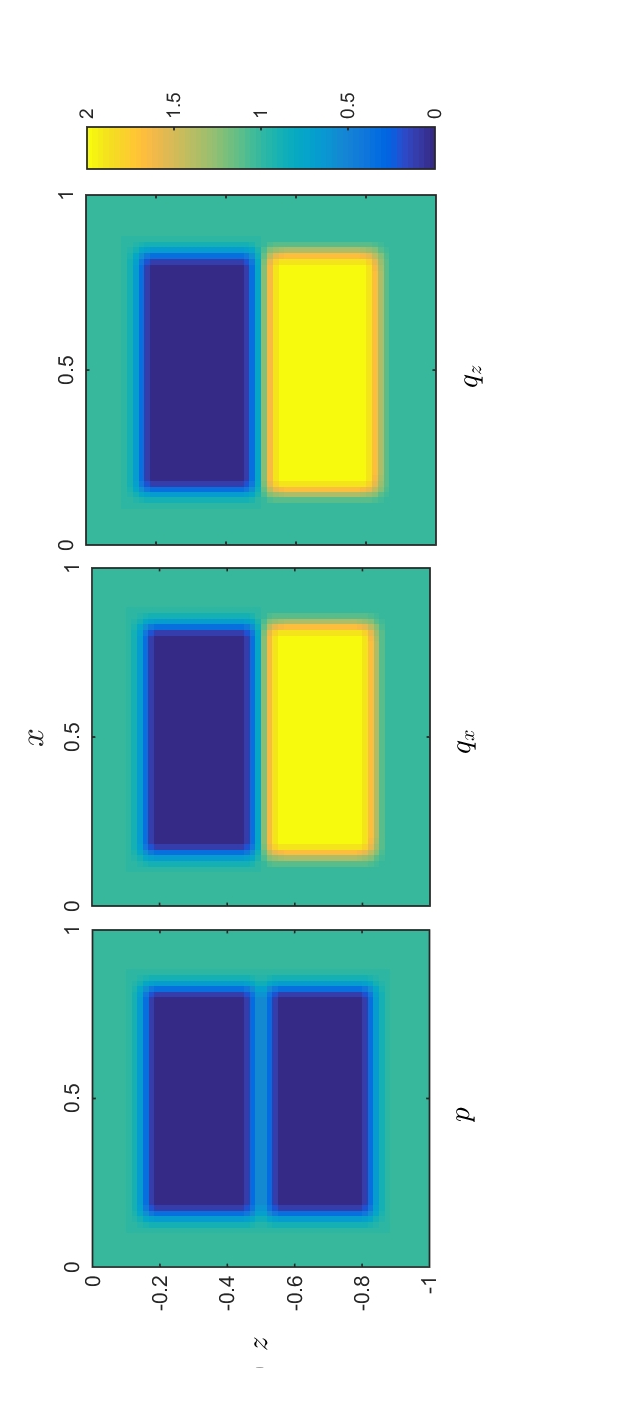
\includegraphics[scale=0.55, angle=270]{2D_Mix_lp_norms}
\caption{Distribution of $l_p$-norm on the model and model gradients over the 2-D model domain. The original boundary of each region was smoothed in order to get a slow transition and reduce visible artifacts. Regions were chosen to cover a larger area than the anomalies to simulate  a blind-inversion. }
\label{fig:2D_Mix_lp_norms}
\end{figure}

\begin{figure}[p]
\centering
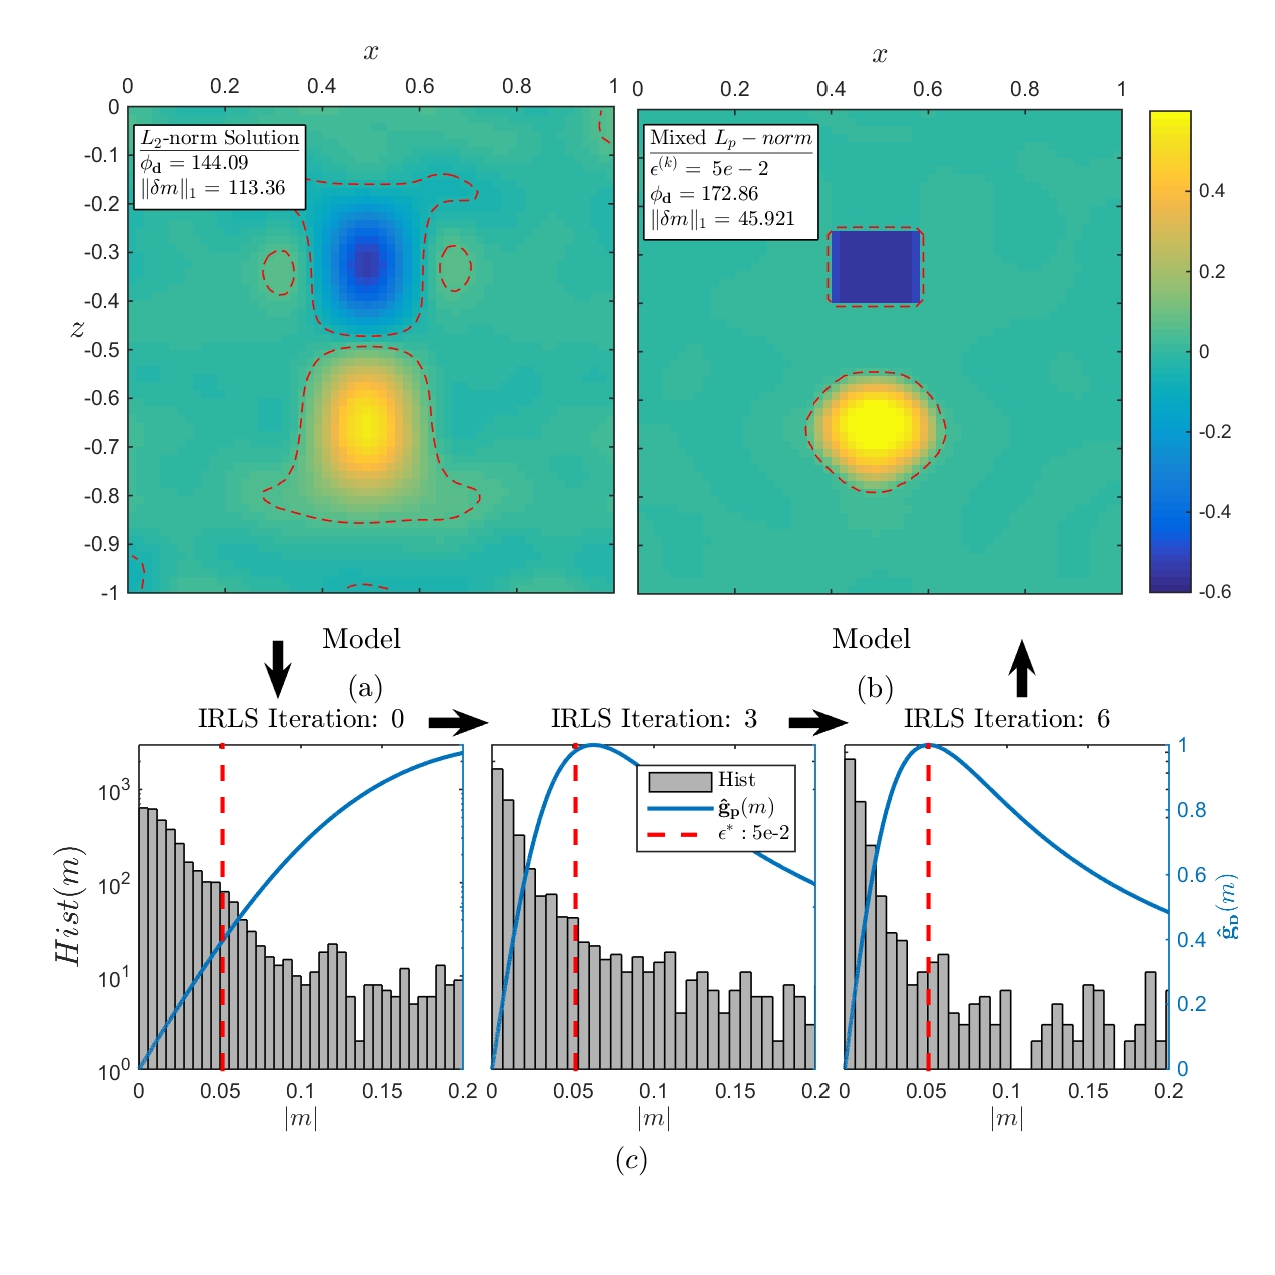
\includegraphics[scale=0.6]{2D_Mix_norm_result}
\caption{(a) Smooth $l_2$-norm solution used to initiate the IRLS iterations. (b) Recovered model using the mixed-norm regularization after seven S-IRLS iterations. The contour line (red) marks the value of $\epsilon_p$, judged to be the \emph{effective zero} value of the model ($m_i \leq $  5e-2). Both models (a) and (b) fit the data within 2\% of the target misfit $\phi_d^*$. (c) Dual plots showing the distribution of model parameters and the gradient of the $l_0$-norm penalty function $\mathbf{\hat g_p}(m)$ as a function of S-IRLS iterations. High penalties are applied to progressively smaller model values.
The final model nicely recovers both the blocky and smooth Gaussian anomaly.}
\label{fig:2D_Mix_norm_result}
\end{figure}


\newpage
\subsection{3-D example}
 As a final test, I invert the same synthetic 3-D susceptibility example as presented in Section \ref{ch:Chap3_MSI}. The model consists of a folded anomaly with magnetic susceptibility of 0.075 SI, arching around a discrete block with susceptibility of 0.05 SI. The arc-shaped anomaly is dipping $20^\circ$ towards the south. 
 
I impose sparsity constraints on the model gradients such that ($p=0,\; q_x=2,\; q_y=2,\; q_z=2$).
 Figure \ref{fig:3D_Inv_l0l2_model_INDUCED} shows the recovered model after five IRLS iterations. The solution is remarkably closer to the true solution, both in shape and model values compared to the smooth $l_2$-norm solution. The inversion also has an easier time reproducing the high frequency content from the data as shown in Figure \ref{fig:3D_Inv_l0l2_pred_INDUCED}. The inversion successfully recovers two distinct objects, no longer connected at depth. Notice that both arms are well defined and extend along the entire length of the arc.
 
As a second experiment, I impose a constraint on the model gradients in order to recover a blocky model.
Model gradients are measured with the standard finite difference operators, expected to yield right-angled anomalies.
Figures~\ref{fig:3D_Inv_l0l0_model_INDUCED} and \ref{fig:3D_Inv_l0l0_pred_INDUCED} show the recovered model and predicted data for $(p = 0,\; q = 1)$, yielding a sparse and blocky solution.
Once gain, compared to the smooth $l_2$-norm solution, the correlated data residuals are substantially reduced.
The recovered susceptibility values within the block and arc shape are more uniform than with the smoothness constraint, ideal to get a bulk estimate in physical property.
 
 \newpage
\begin{figure}[h!]
\centering
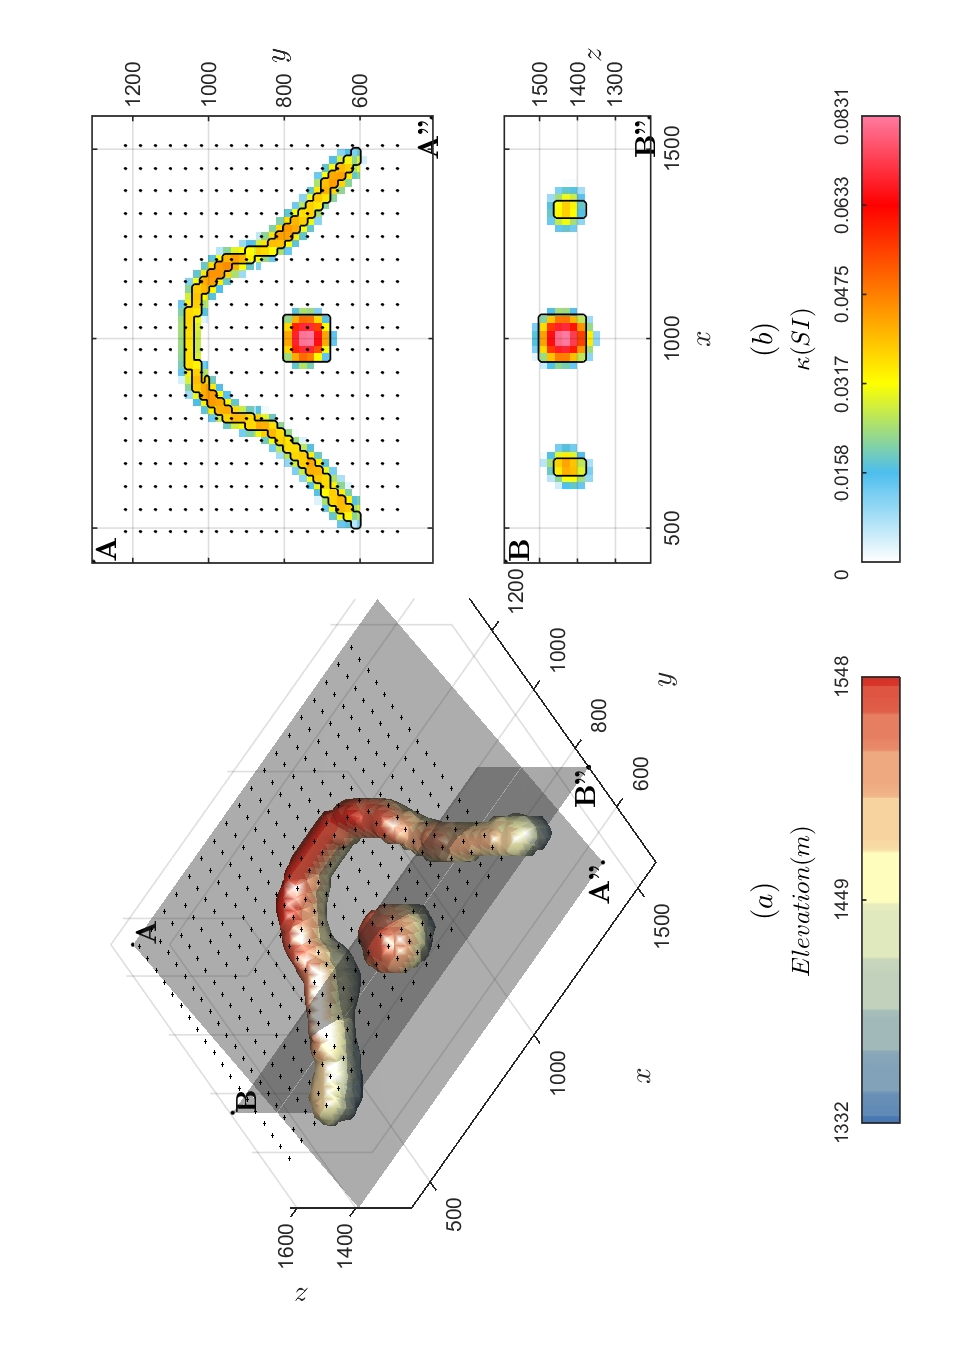
\includegraphics[scale=0.52, angle =270]{3D_Inv_l0l2_model_INDUCED.pdf}
\caption{ (a) Iso-surface (0.002 SI) and (b) sections through the recovered susceptibility model after five IRLS iterations for $(p = 0,\; q = 2)$. The final model is substantially closer to the true solution.}
\label{fig:3D_Inv_l0l2_model_INDUCED}
\end{figure}
\begin{figure}[h!]
\centering
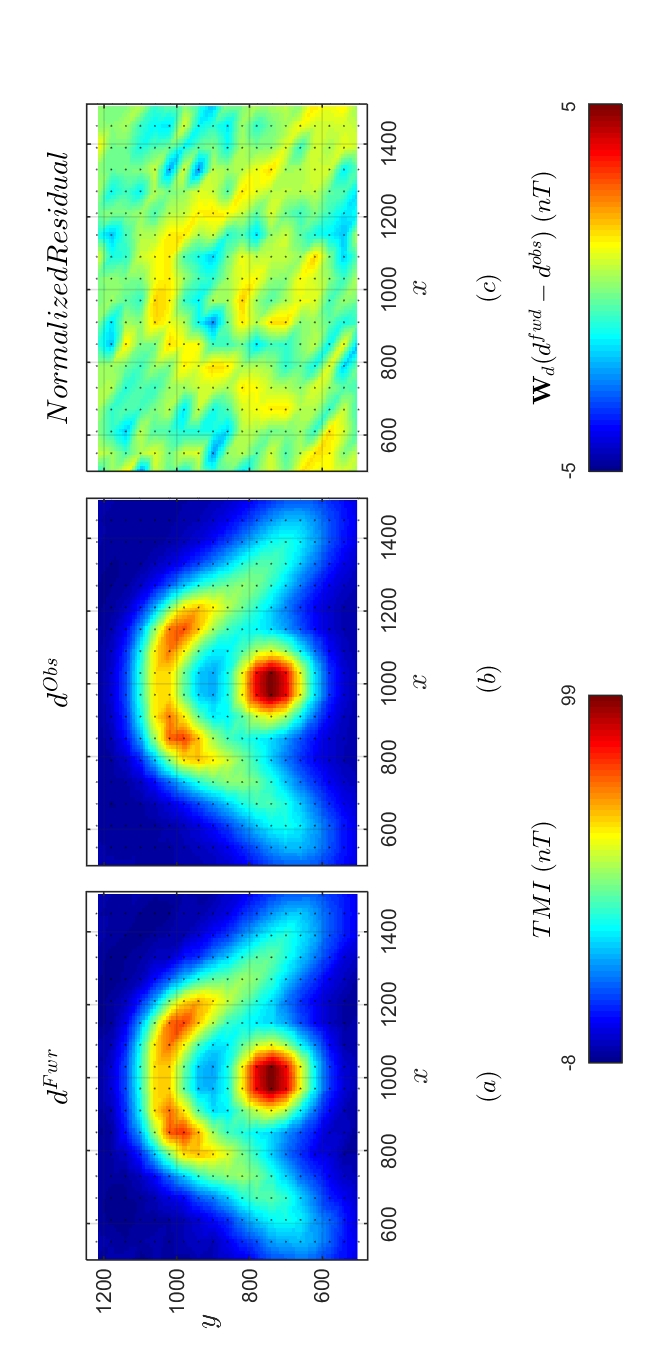
\includegraphics[scale=0.52, angle =270]{3D_Inv_l0l2_pred_INDUCED.pdf}
\caption{ Comparison between (a) observed and (b) predicted data from the recovered susceptibility model using compact norms for  $(p = 0,\; q = 2)$. (c) Normalized data residuals are within two standard deviations.}
\label{fig:3D_Inv_l0l2_pred_INDUCED}
\end{figure}

\newpage
\begin{figure}[h!]
\centering
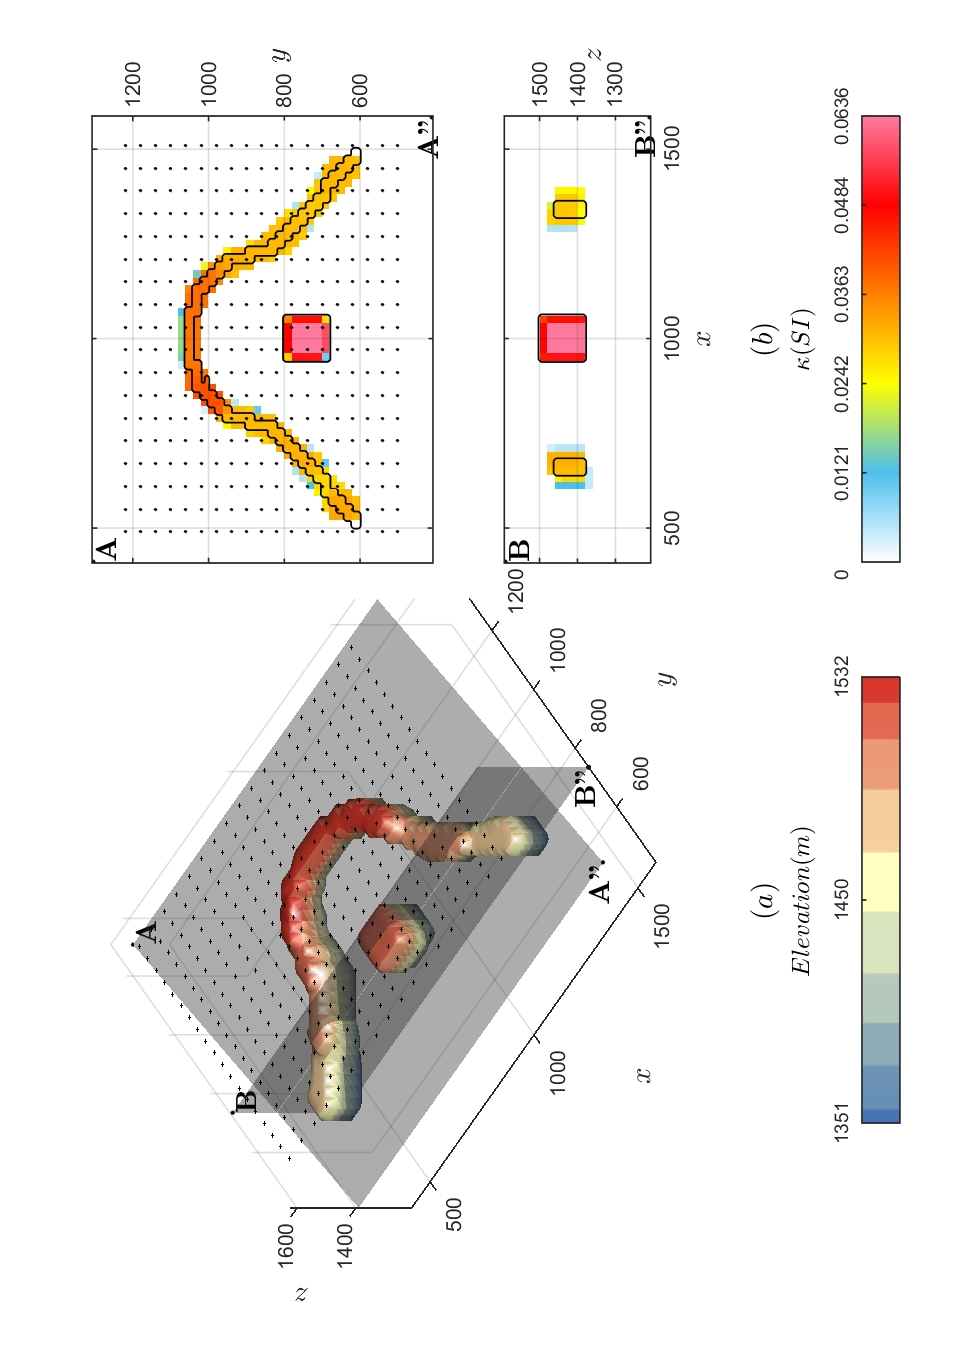
\includegraphics[scale=0.52, angle =270]{3D_Inv_l0l0_model_INDUCED.pdf}
\caption{ (a) Iso-surface (0.002 SI) and (b) sections through the recovered susceptibility model after nine IRLS iterations for $(p = 0,\; q = 1)$ . Sparsity constraints on the model and model gradients yield a simple and blocky model.}
\label{fig:3D_Inv_l0l0_model_INDUCED}
\end{figure}
\begin{figure}[h!]
\centering
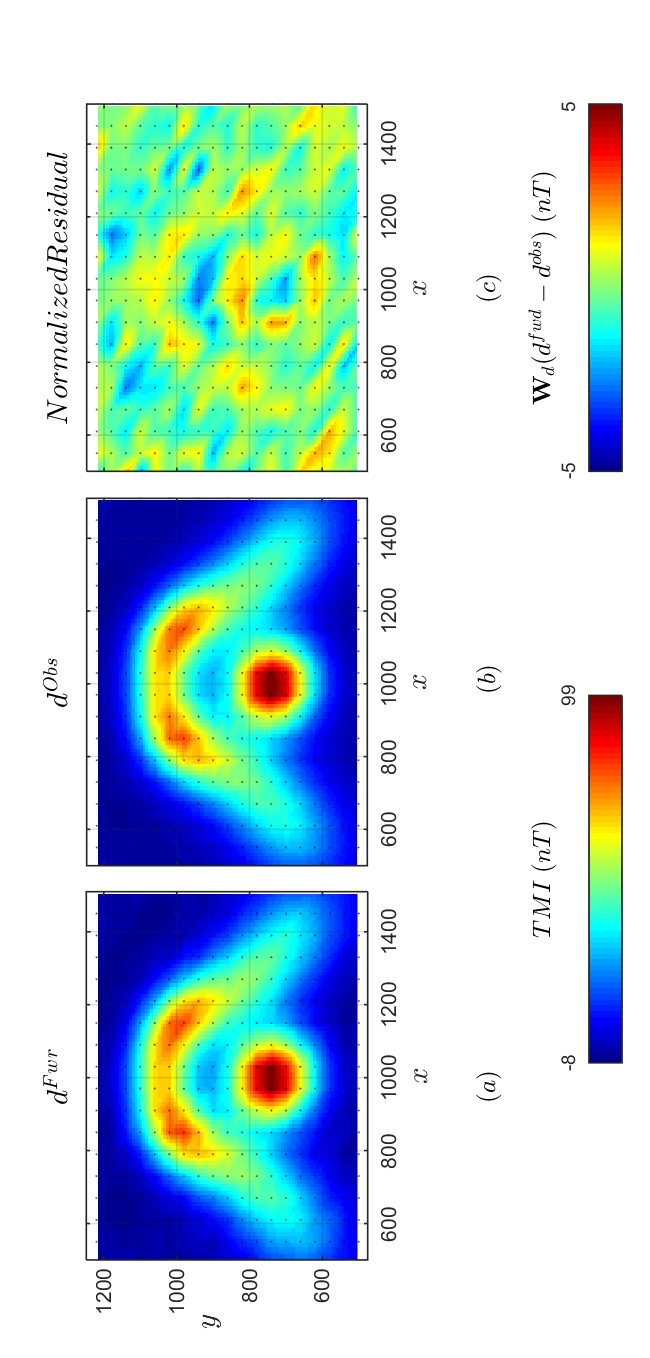
\includegraphics[scale=0.52, angle =270]{3D_Inv_l0l0_pred_INDUCED.pdf}
\caption{ Comparison between (a) observed and (b) predicted data from the recovered susceptibility model using compact norms for  $(p = 0,\; q = 1)$. (c) Normalized data residuals are within two standard deviations.}
\label{fig:3D_Inv_l0l0_pred_INDUCED}
\end{figure}

\section{Case study - Tli Kwi Cho kimberlite complex}\label{3D_Section}
As a final test, I apply the mixed-norm S-IRLS algorithm on a magnetic data from the Tli Kwi Cho (TKC) diamondiferous kimberlite complex.
The property is located in the Lac de Gras region,  approximately 350 km northeast of Yellowknife, Northwest Territories, Canada.
The TKC deposit was originally discovered by an airborne DIGHEM survey in 1992, including frequency-domain EM and magnetic data. 
Two kimberlite pipes, dubbed DO27 and DO18, were later confirmed by drilling in 1993.  
Different volcaniclastic rock units suggests that the deposit was formed over several events \cite[]{DoyleEtAl1999}. 
The pipes are intruding into older granitic rocks of the Archean Slave Province, known to have little to no magnetite content.
A magnetic susceptibility contrast between the kimberlite and the country rocks give rise to noticeable anomalies on the observed TMA data.
Strong linear features associated with the Mackenzie dyke swarms can be observed on the eastern part of the survey.
These dykes extend over the entire Lac de Gras region and generally strike $305^\circ$N \cite[]{Wilkinson2001}. 
They are known to be near vertical and are typically between 20-50 m wide. 
This geological setting is therefore ideal for implementing a mixed-norm algorithm. 
My goal is to apply \emph{soft} constraints on the model values and model gradients in order to favor specific geometry. 

Prior to the inversion, I rotate the regional dataset by $30^{\circ}$ counterclockwise to a local coordinate system in order to align the principal axis of the dykes parallel to the grid. 
The declination of the inducing field are also rotated by $30^\circ$ to preserve the geometry of the problem.
The region of interest is discretized into 25 m cube cells.
In preparation for Phase II of the S-IRLS algorithm, a smooth solution is found with the $l_2$-norm regularization as shown in Figure \ref{fig:TKC_Mag_Models}(a).
The inversion recovers two discrete bodies corresponding to the known location of DO18 and DO27.
Two linear anomalies striking north-south correspond with the Mackenzie dyke swarms. A third anomaly intersects at right-angle running $90^{\circ}$N.
As expected from the $l_2$-norm regularization, the solution is smooth and edges are not clearly defined.
Note also that the highest recovered susceptibilities are strongly correlated with the observation locations.
Dykes appear to break up between each survey line, which is clearly an inversion artifact due to changes in sensitivities. 

I want to modify the objective function in order to recover sharp and continuous edges.
In general terms, I want to enforce large gradients perpendicular to the strike of the dykes, while imposing a sparsity constraint over the kimberlite pipes.
I divide the region of interest into four sub-regions as shown in Figure \ref{fig:TKC_Mix_Norm}:
\begin{itemize}
\item{$S_1$: Sub-region covering the Mackenzie dyke swarms on the eastern edge of the survey. 
I impose an $l_0$-norm on the model gradients in the $\hat x$-direction ($q_x = 0$) to get sharp edges along the strike of the dykes, but smooth in the other directions ($q_y, q_z, p = 2$). }
\item{$S_2$: Sub-region covering the dyke running perpendicular to  the Mackenzie dyke swarms. Similar to $S_1$, I impose an $l_0$-norm on the model gradients in the $\hat y$-direction ($q_y = 0$). }
\item{$S_3$: Sub-region covering the kimberlite pipes DO27 and DO18. I impose an $l_1$-norm on the model gradients ($q_x, q_y, q_z = 1$) and an $l_0$-norm on model value ($p=0$) in order to recover blocky and sparse anomalies. }
\item{$S_4$: Background region covering the rest of the survey area. I impose an $l_2$-norm on the model gradients ($q_x, q_y, q_z = 2$) and an $l_1$-norm on model value  ($p=1$) in order to recover a smooth and sparse model. }
\end{itemize}

Figure \ref{fig:TKC_Mag_Models}(b) presents the recovered model obtained after five iterations of the S-IRLS algorithm. 
In comparison with the smooth inversion, the edges of all three dykes are better defined and extend vertically at depth. 
The inversion may suggest the presence of a fourth dyke parallel to the Mackenzie dyke swarm, on the eastern edge of the survey.
Both DO18 and DO27 are recovered as compact bodies with higher susceptibility and well defined edges compared to the smooth $l_2$-norm inversion. 
Because of the small $l_0$-norm applied to model values, most of the near surface anomalies are removed, yielding a more compact anomaly at depth.
This is also true away from the kimberlite pipe over the background region, where a simpler model is obtained.
Predicted data for the smooth $l_2$-norm model and the final S-IRLS solution are presented in Figure \ref{fig:TKC_Obs_vs_Pred}, both within $5\%$ of the target misfit.

\begin{figure}[p]
\centering
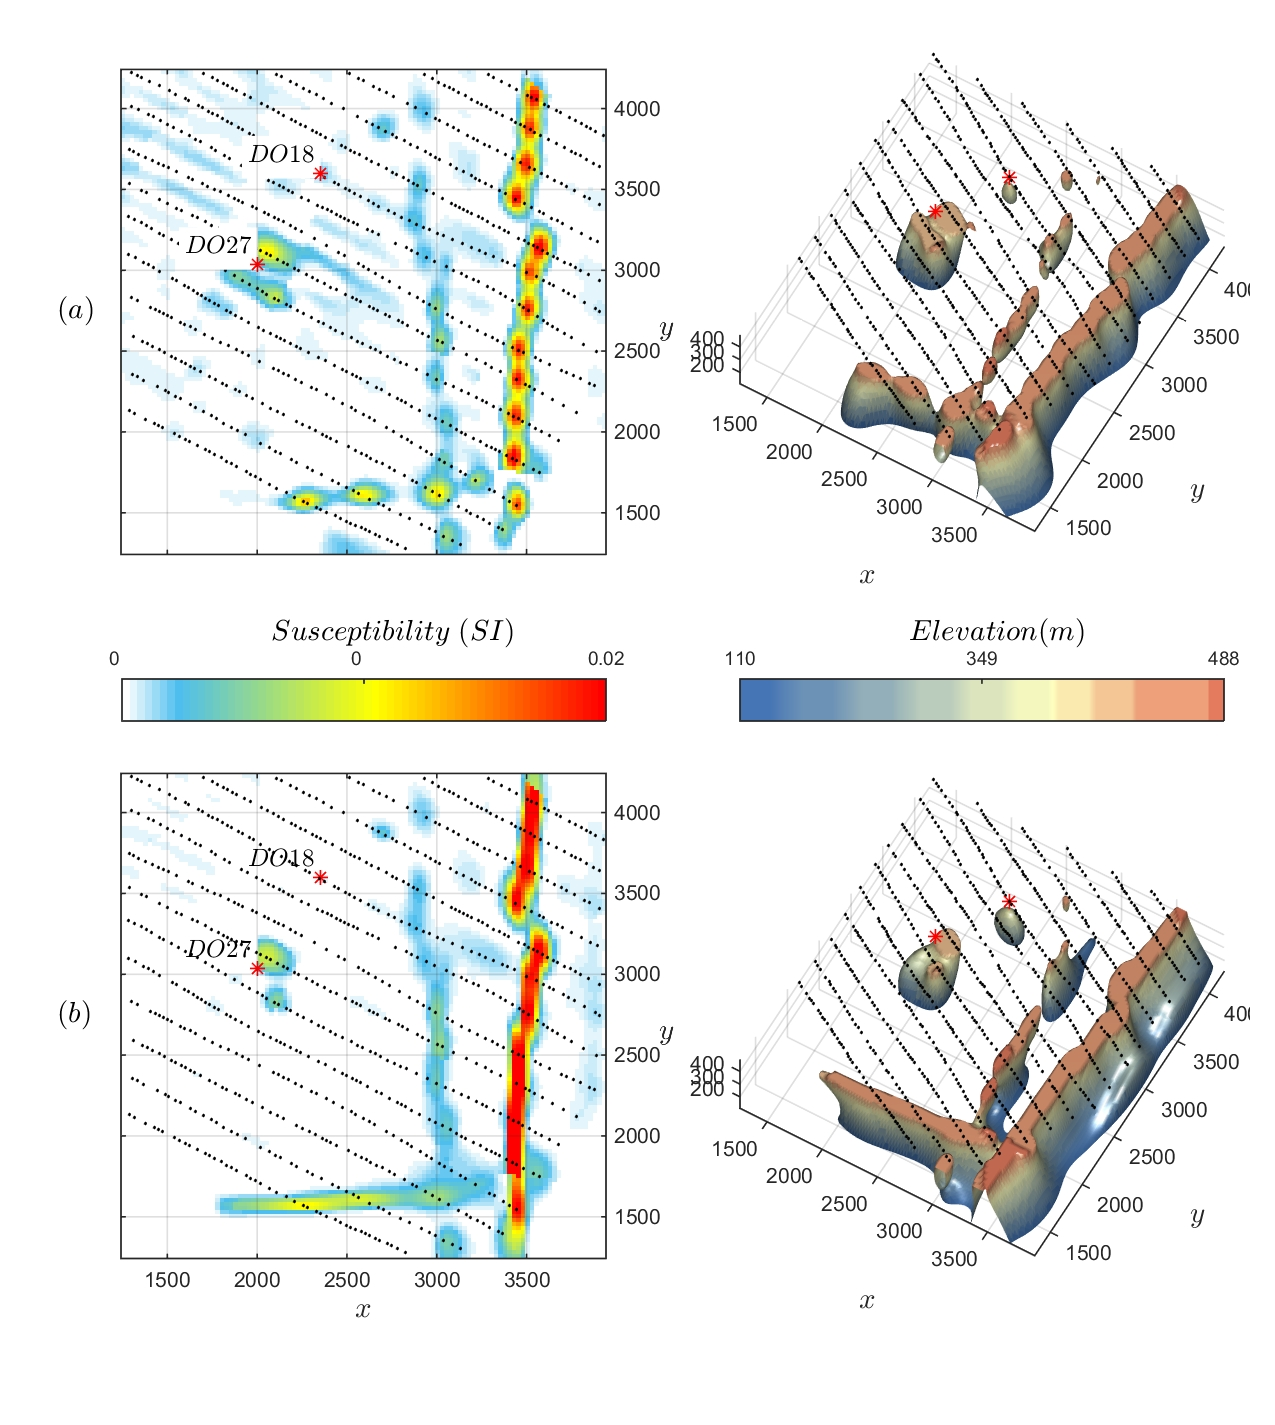
\includegraphics[scale=0.60]{TKC_Mag_Models}
\caption{(a) (Left) Horizontal section through the recovered susceptibility model at 25 m depth below topography from the smooth $l_2$-norm regularization. (Right) Iso-surface of susceptibility values around 0.002 SI.
(b) Recovered model using the mixed-norm S-IRLS algorithm. Magnetic dykes are better recovered, imaged as continuous plates and extending vertically at depth. Susceptibility values for DO-27 and DO-18 have increased, showing as compact vertical pipes.}
\label{fig:TKC_Mag_Models}
\end{figure}

\begin{figure}[p]
\centering
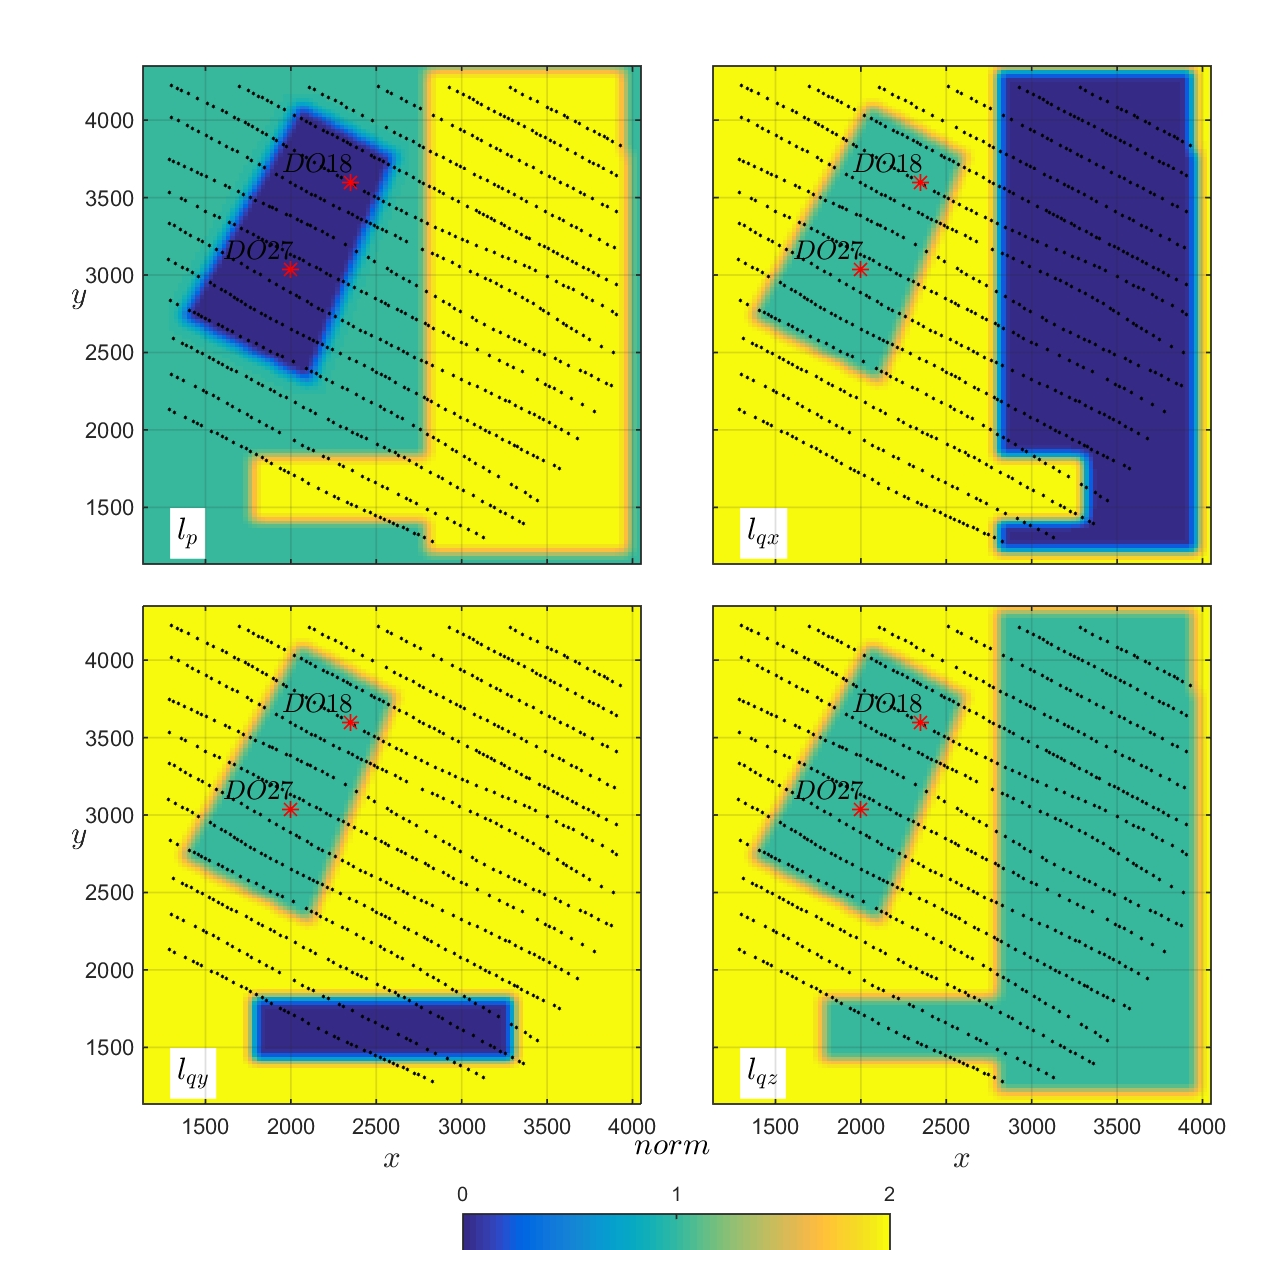
\includegraphics[scale=0.60]{TKC_Mix_Norm.pdf}
\caption{Horizontal section through the mixed-norm models applied to four sub-regions with smooth transition across zones.}
\label{fig:TKC_Mix_Norm}
\end{figure}

\begin{figure}[p]
\centering
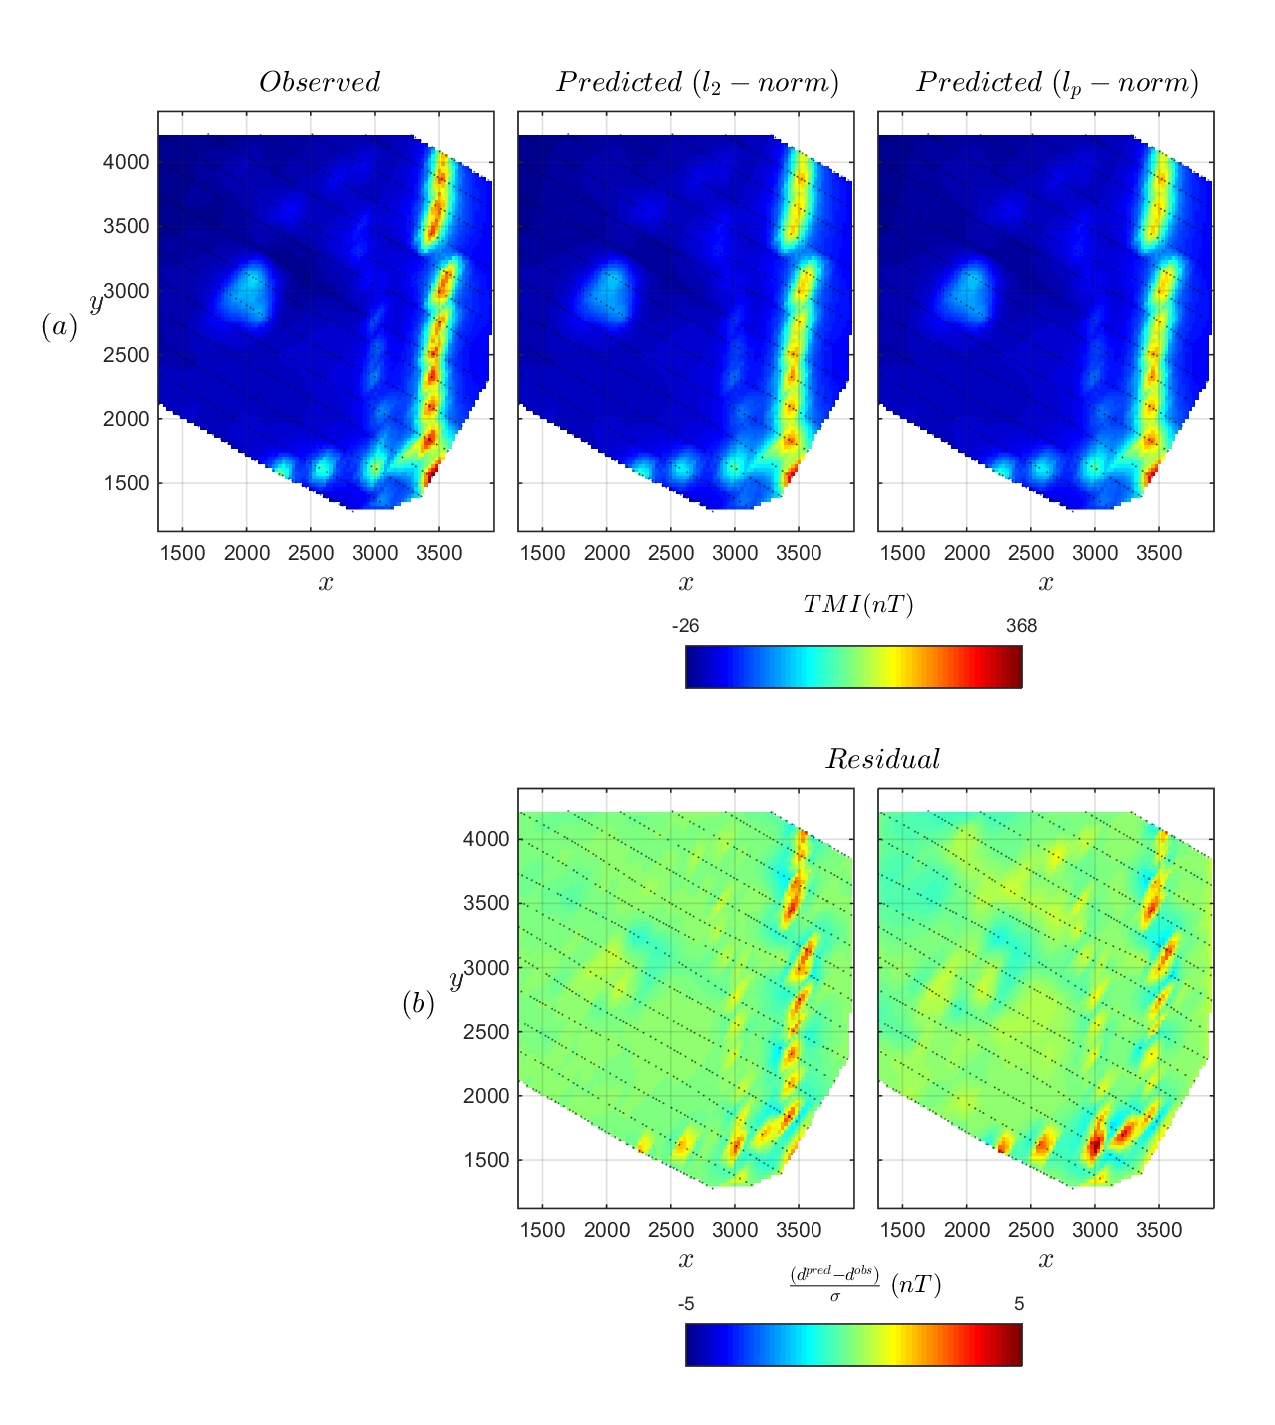
\includegraphics[scale=0.60]{TKC_Obs_vs_Pred.pdf}
\caption{(a) Observed and predicted data over the TKC kimberlite complex. (b) Residuals between observed and predicted data normalized by the estimated uncertainties (10 nT). Both the smooth and mixed-norm inversions reproduce the data within four standard deviations.}
\label{fig:TKC_Obs_vs_Pred}
\end{figure}


%\newpage
\section{Summary}
In this chapter, I reviewed and experimented with several algorithms for the approximation of $l_p$-norm measures on the model and model gradients to promote sparse and blocky solutions. 
I proposed a Scaled-IRLS algorithm in order to stabilize current inversion strategies, while reducing the computational cost. 
My algorithm offers a strategy to determine an optimal value for the stabilizing parameter $\epsilon$, previously overlooked by other researchers. This robust method is further generalized, allowing for mixed-norm penalties on the model and model gradients. Scalings are applied to the individual terms of the regularization function in order to preserve their relative importance during the inverse process. 
A solution to the non-linear inverse problem is found iteratively using Gauss-Newton steps. 

Varying the combination of $l_p$-norm of the model and its gradients allows me to shape the objective function to exhibit specific characteristics. For different geological settings, there is likely a specific combination of norms that can better recover the true geometry of causative bodies. 
Preliminary results show great promise at reducing the non-uniqueness of current potential fields inversion codes.
Because my formulation is general, the algorithm can be applied to a wide range of inverse problems. 


\endinput

